\PassOptionsToPackage{quiet}{fontspec}
\documentclass[12pt,a4paper,UTF8]{article}
\usepackage{thesis} % 格式控制
\usepackage{indentfirst}
\usepackage{enumitem}
\usepackage{float}
\usepackage{array}
\usepackage{longtable}
\usepackage{xltabular}
\usepackage{etoolbox}


\setlength{\parindent}{2em} % 控制首行缩进  
\addtolength{\parskip}{3pt} % 控制段落距离  
\onehalfspacing % 1.5倍行距  
\graphicspath{{./figures/}} % 指定图片所在文件夹  


\classname{软件工程}  % 设置课程名称
\makepagestyle{}{\printclassname ~:需求分析书}




\begin{document}
\maketitlepage{需求分析书}{动物领养系统}{尹建伟}{计算机科学与技术学院}{}{}{} 

\maketoc    %目录页

\section{引言}

本章为说明本需求报告的编写目的及介绍本项目的相关背景。 

\subsection{编写目的}

本需求分析旨在详尽分析动物领养系统的需求,描述系统提供的功能以及服务。本需求分析的预期读者包括需求提出方,系统架构师,软件工程师,测试工程师以及 \verb|UI| 设计师。

本需求分析是在系统开发前期用于的需求,描述模块所提供的功能和性能,确定模块的参数和属性。本需求分说明的预期读者包括需求提出方和软件开发者。为了提供软件设计的基础,模块的不同需求会被详细分析,同时所提供的相应功能也将被阐明。

\subsection{相关背景}

\begin{itemize}
  \item 软件系统名称:\verb|ChaMaoMao|
  \item 任务提出者:吴岱阳
  \item 开发者:吴岱阳,金俊一,鲁悦,季海川,陶卓
  \item 用户:主要面向浙大以及社会的动物爱好者,动保组织
  \item 实现该软件的计算机网络:公开网络
\end{itemize}

浙江大学软件工程基础课程分为理论课和实践课两部分。在理论课中,教师有选择地介绍了与软件工程相关的基本理论,并强调和确定了适用于整个软件生命期的基本原则,全面而深入地介绍了这些基本原则在软件设计、规范、验证、软件生产过程和管理活动中的运用。在实验课中,课程采取分组形式完成,每组学生分为 \verb|Project Manager|、\verb|UI Designer|、\verb|Database Designer|、\verb|Testing|、\verb|Software Configuration Manager|、\\ \verb|Document and SQA Manager| 几个角色,按照不同的角色分工完成最终的项目工程。

在本次课程中,本项目组选择动物领养系统作为综合性实验题目。

\subsection{名词解释}

本需求分析书中会出现部分软件工程开发的专业术语,为方便读者理解后续内容,将部分术语解释如下:

\begin{itemize}
  \item \verb|CRC|
\end{itemize}

英文全拼为 \verb|Class-Responsibility-Collaborator|,翻译为 “类-职责-协作人”,即表示一个类、类的职责以及类的协作关系。它是比较流行的一种面向对象分析建模方式。类表示一系列对象的集合,这些对象是对系统设计的抽象建模,可以是一个人、一件物品等等。类名写在 \verb|CRC| 卡的最上方,职责包括这个类对自身信息的了解,已经这些信息将如何应用。诸如,一个人,他知道他的电话号码、地址、性别等属性,并且他知道他可以说话、行走的行为能力,这个部分在 \verb|CRC| 卡的左边。协作代指另外一个类,我们可以通过这个类获取我们想要的信息或者相关操作,这个部分在 \verb|CRC| 卡的右边。

\begin{itemize}
  \item 数据流图
\end{itemize}

数据流图是结构化分析方法中使用的工具,它以图形的方式描绘数据在系统中流动和处理的过程,由于它只反映系统必须完成的逻辑功能,所以它是一种功能模型。在结构化开发方法中,数据流图是需求分析阶段产生的结果。数据流图从数据传递和加工的角度,以图形的方式刻画数据流从输入到输出的移动变换过程。

\begin{itemize}
  \item 状态图
\end{itemize}

状态图是描述一个实体基于事件反应的动态行为,显示了该实体如何根据当前所处的状态对不同的事件做出反应。通常我们创建一个 \verb|UML| 状态图是为了以下的研究目的:研究类、角色、子系统、或组件的复杂行为。而状态图用于显示状态机(它指定对象所在的状态序列)、使对象达到这些状态的事件和条件、以及达到这些状态时所发生的操作。

\section{项目简介}

\subsection{项目提出与意义}

领养代替购买是这些年被很多人认可并且推广的一种养宠概念,这个理念的核心是通过领养的方式给流浪动物或被公益组织收容的宠物提供一个家。但是在实际生活中人们对于领养宠物的认知和态度并不完全一致。据调查显示,\verb|43.9%| 的宠物狗是从宠物店获得的,而领养的狗占比 \verb|11.8%|,宠物猫的来源除了街上捡到的 \verb|32.6%|,宠物店购买的占比 \verb|25.3%|,而领养的占比仅仅为 \verb|19.9%| 的比例。

除此之外,根据世卫组织的数据,目前世界上有超过两亿只流浪动物。其中,我国的流浪动物数量占据四千多万只。根据宠物消费趋势白皮书,我国的宠物行业市场规模接近三千亿元,未来行业也将继续保持稳定增长,复合增长率为 \verb|14.2%|,我国的宠物消费市场前景非常广阔。

在浙江大学中也有许多的流浪动物,以猫咪居多。为了帮助这些流浪动物找到一个温暖的家,\verb|ChaMaoMao| 这个以流浪动物领养为主的项目应运而生。我们希望通过这个项目能够帮助更多的流浪动物找到一个温暖的家。

通过动物领养系统,动物保护组织可以更有效地管理和运作。系统化的记录和管理工具可以提高组织的工作效率,减少人力和时间成本。而系统中的透明度和可追溯性,可以增加公众对组织的信任,并吸引更多人参与宠物救助和领养的活动。该系统的建立不仅有助于提高宠物福利,促进宠物领养,减少流浪问题,还可以推动社会对动物保护的意识和行动。这对于构建和谐社会、提升公共文明素质具有重要意义。

\subsection{项目具体内容介绍}

\begin{figure}[!htbp]
  \centering
  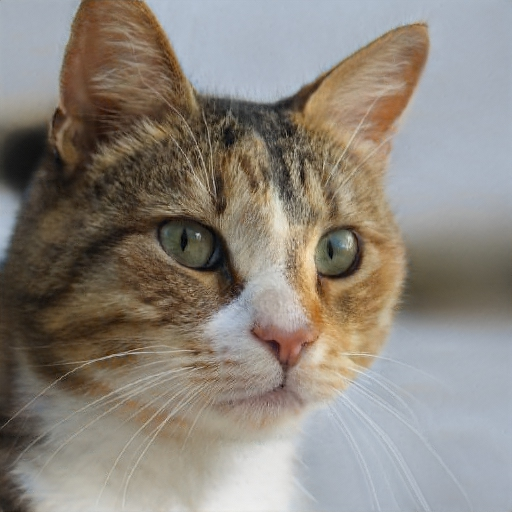
\includegraphics[width=0.25\textwidth]{figures/example.png}
\end{figure}

动物领养系统主要着眼于以下功能:动物爱好者和用户的管理、动物信息的管理、领养处理、动物定位、动物识图搜索、领养教程和指南的发布等。在本动物领养平台上,用户可以注册账号,关注自己喜欢的动物,查看相关动物信息,提出领养请求,实现自己的养宠梦想;动保管理员负责审核用户信息,发布和审核领养信息,维护动物具体信息,发布领养教程和指南等。

\subsection{产品市场分析}

\subsubsection{国内市场分析}

在调查过程中,我们发现在关于宠物领养的网站和平台中,已经有一些成熟的产品在市场占据了一定份额,但其在采取的功能和开发商业存在一定的差异。

\begin{figure}[!htbp]
  \centering
  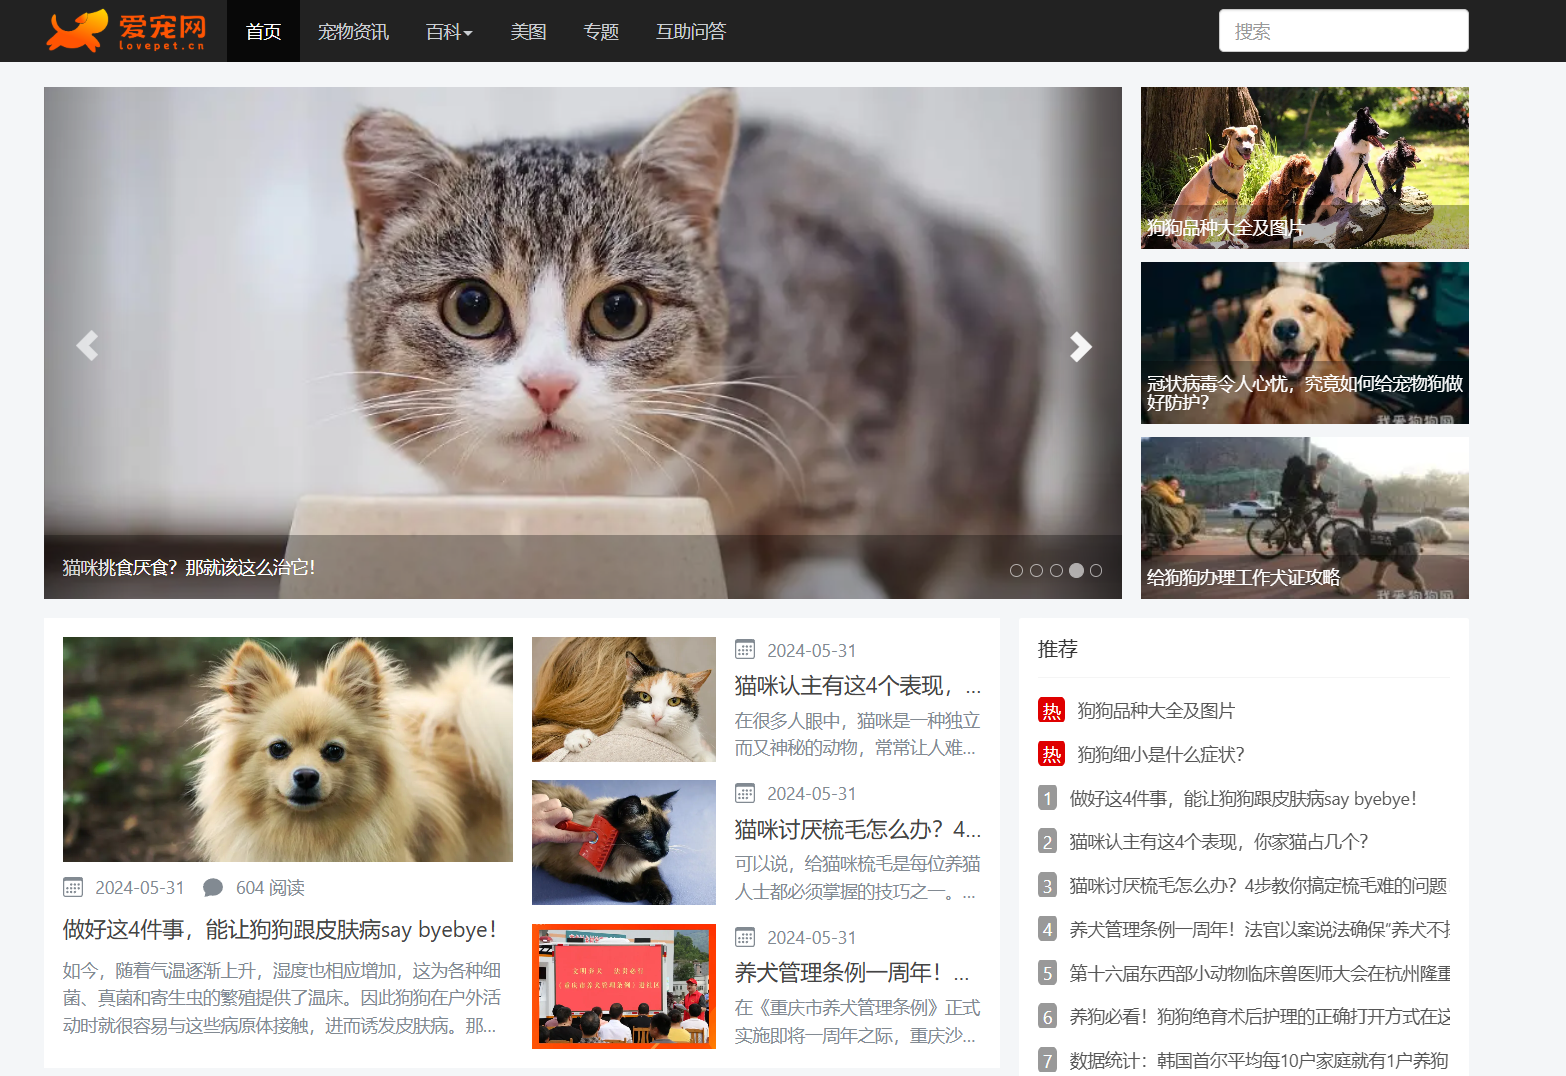
\includegraphics[width=0.6\textwidth]{figures/lovepetcn.png}
\end{figure}

以爱宠网为例,其是一个非常可靠的宠物平台,可以为用户提供一些领养宠物信息和机构的联系方式。但其更偏向于一个宠物知识展示和团队交流平台,对于领养功能实现并不完全,且领养内容较少,在首页很难找到相关的领养入口。

\begin{figure}[!htbp]
  \centering
  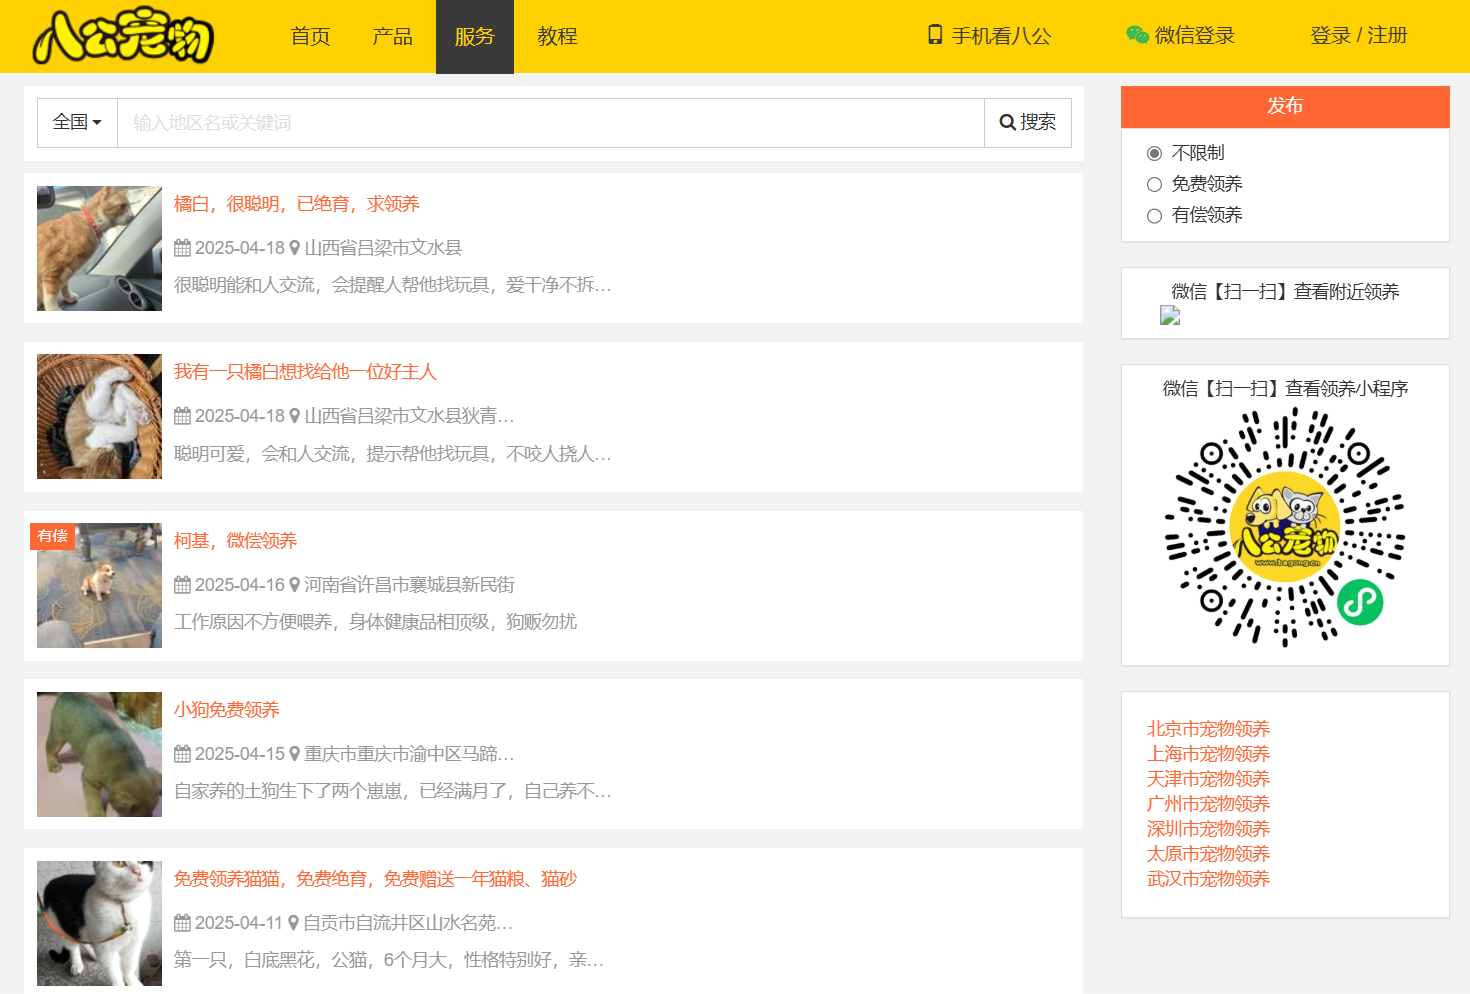
\includegraphics[width=0.7\textwidth]{figures/bagongpet.png}
\end{figure}

而另一个网站:八公宠物。其更倾向于是为宠物找寻领养家庭的平台,普遍是用户为自家宠物寻找领养家庭,而不是流浪动物。其在宠物领养方面的功能也并不完善,交互界面比较简单,内容较少且索引较差。

当然,还有一些热门的社交媒体和软件,如小红书、微博、抖音上都有很多的宠物领养信息,但其并不是专门的宠物领养平台,用户在使用时需要花费大量的时间去寻找相关的信息。还有很多的宠物领养都是依靠某地的动保组织或者是有爱心的宠物店进行的,而不是专门的一个线上平台或软件。

\subsubsection{国外市场分析}

\begin{figure}[!htbp]
  \centering
  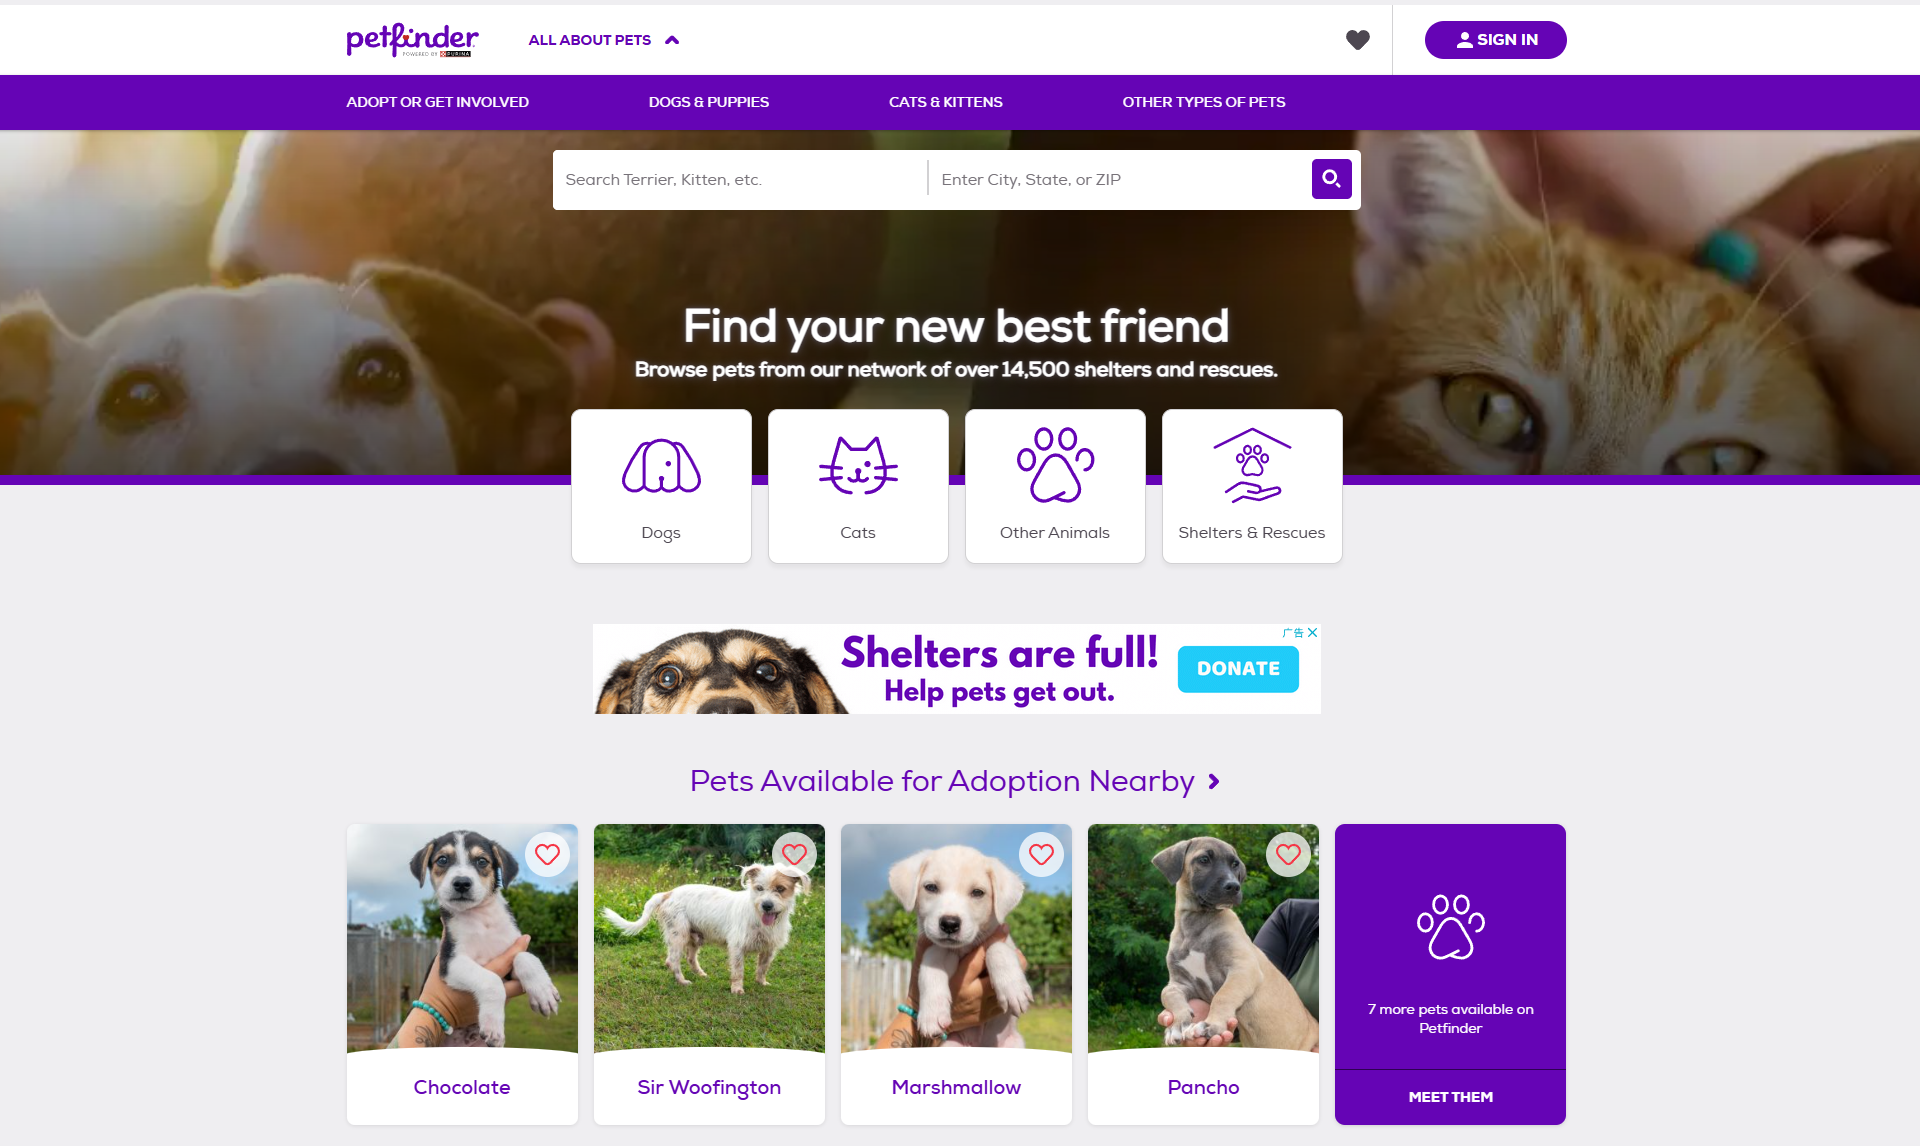
\includegraphics[width=0.7\textwidth]{figures/petfinder.png}
\end{figure}

国外也有类似的平台,如 \verb|Petfinder| 和 \verb|Adoptapet| 等。它们都比较成熟且出名,拥有大量的用户和宠物信息。

\verb|Petfinder| 拥有数百万条宠物领养信息,涵盖了各种类型的宠物,包括狗、猫、兔子、鸟类等。其功能强大,用户可以根据地理位置、宠物类型、品种、年龄等多个条件进行搜索,快速找到心仪的宠物。同时,平台还提供了宠物救助组织的详细信息和评价系统,帮助用户选择可靠的救助组织进行领养。

而 \verb|Adoptapet| 是一个非营利性的动物领养平台,致力于连接流浪动物救助组织和潜在的领养者。该平台界面友好,操作简单,用户可以轻松浏览待领养动物的照片和介绍,并与救助组织工作人员进行在线交流。其还注重领养后的跟踪服务,通过用户反馈和评价机制,确保领养宠物能够得到良好的照顾。

当然,通过对比发现,这些宠物领域系统和平台无论国内外和功能,其核心内容都大同小异,这也是我们在本项目中所要实现的功能。除此之外,对比之下可以容易看出平台的设计风格和交互
友好性也很重要,这些都是我们在开发过程中会重点关注的部分。



\subsection{用户需求}

本节将根据用户提出的需求描述系统的功能,以下为各类用户的需求:

\vspace{0.25cm} % 添加垂直间距

\noindent\textbf{普通用户}:

\begin{itemize}[topsep=2pt, partopsep=0pt]
  \item 注册和登陆用户账号
  \item 修改个人相关信息
  \item 查看动物详细信息
  \item 新建动物、上传照片
  \item 提出领养申请
  \item 查看动物定位地图与更新定位
  \item 动物识图搜索
  \item 查看教程和指南
\end{itemize}

\vspace{0.25cm} % 添加垂直间距

\noindent\textbf{动保管理员}:

\begin{itemize}
  \item 注册和登陆管理员账号
  \item 审核和管理用户信息
  \item 查看动物详细信息
  \item 新建动物、上传照片、编辑动物信息
  \item 发布动物领养信息
  \item 审核动物领养申请
  \item 查看动物定位地图与更新定位
  \item 动物识图搜索
  \item 发布领养教程和指南
\end{itemize}


\section{用户场景}

\subsection{用例图}

\subsubsection{基础信息模块用例图}

\begin{figure}[H]
  \centering
  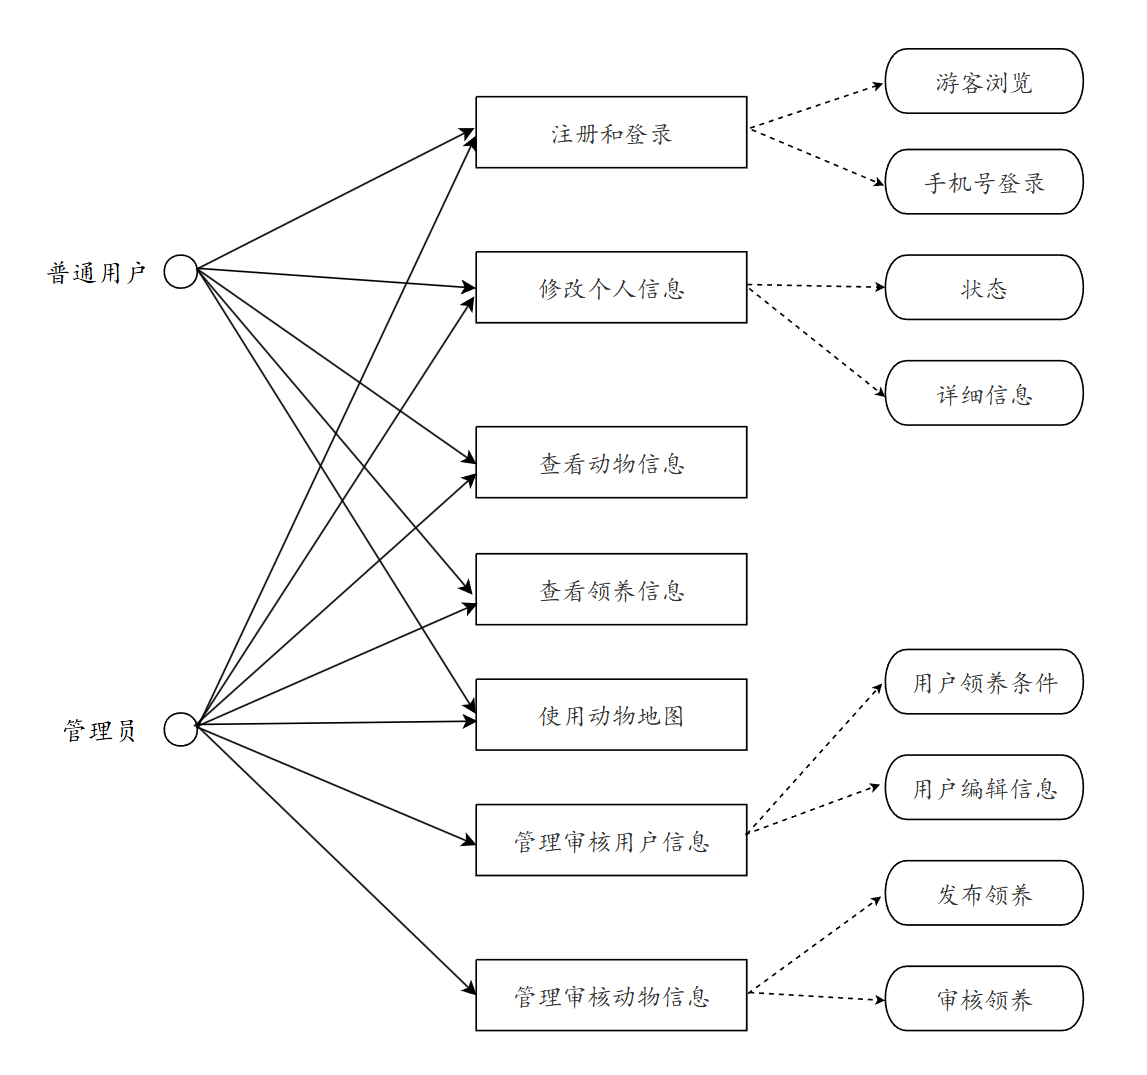
\includegraphics[width=0.9\textwidth]{figures/case1.png}
\end{figure}

\subsubsection{动物领养申请模块用例图}

\begin{figure}[H]
  \centering
  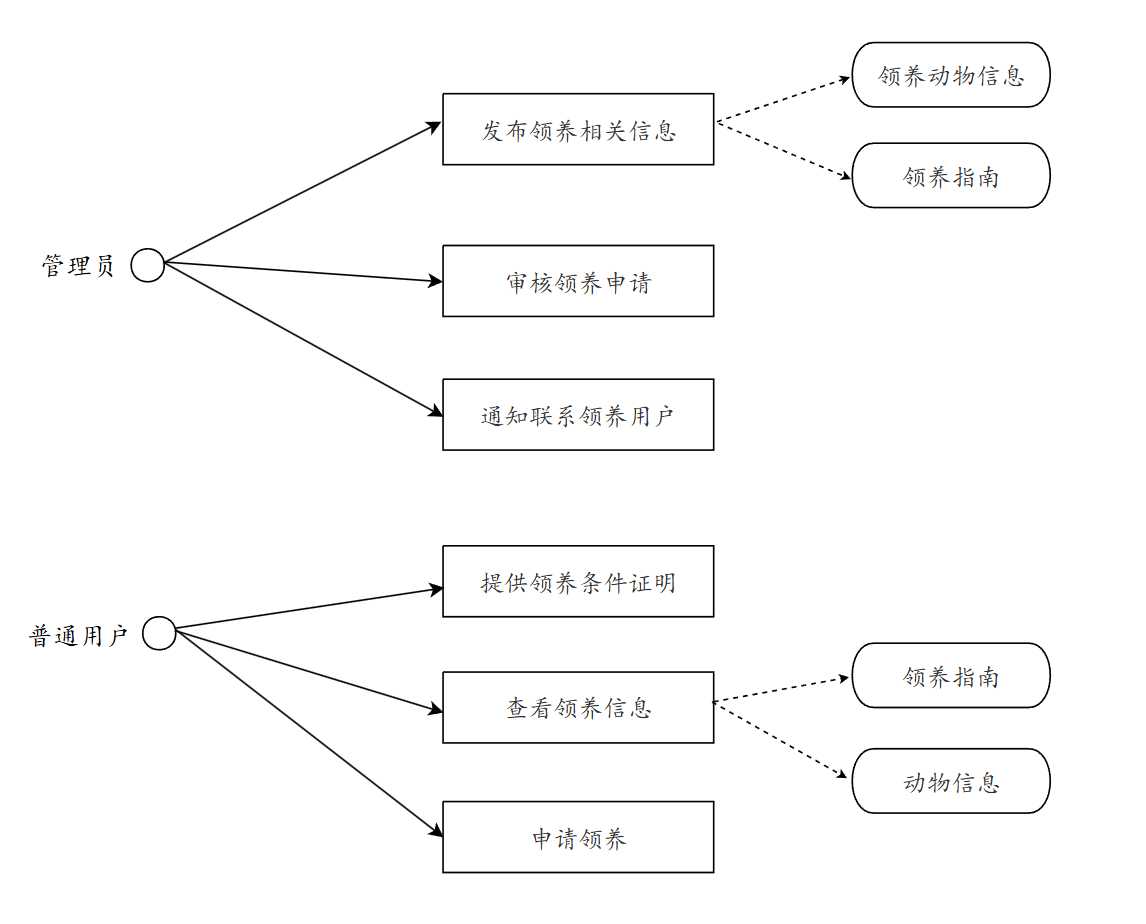
\includegraphics[width=0.9\textwidth]{figures/case2.png}
\end{figure}

\subsubsection{动物地图定位模块用例图}

\begin{figure}[H]
  \centering
  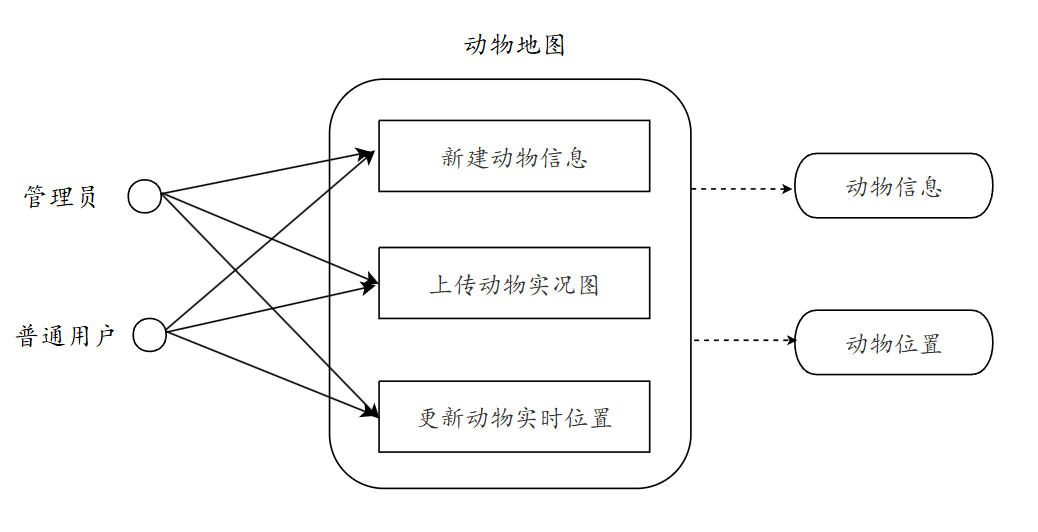
\includegraphics[width=0.9\textwidth]{figures/case3.png}
\end{figure}

\subsection{功能列表}

\subsubsection{用户注册}

\noindent\textbf{描述及优先级}

用户在使用此动物领域系统时需先注册一个账号。注册方式采用手机号登录。系统将根据手机号信息返回注册消息,用户可自由创建个人账号。注册成功后,用户可使用手机号和密码登录系统。

优先级:极高(系统基础功能,必须实现)

\noindent\textbf{主要流程请求/响应时序图}

\begin{figure}[H]
  \centering
  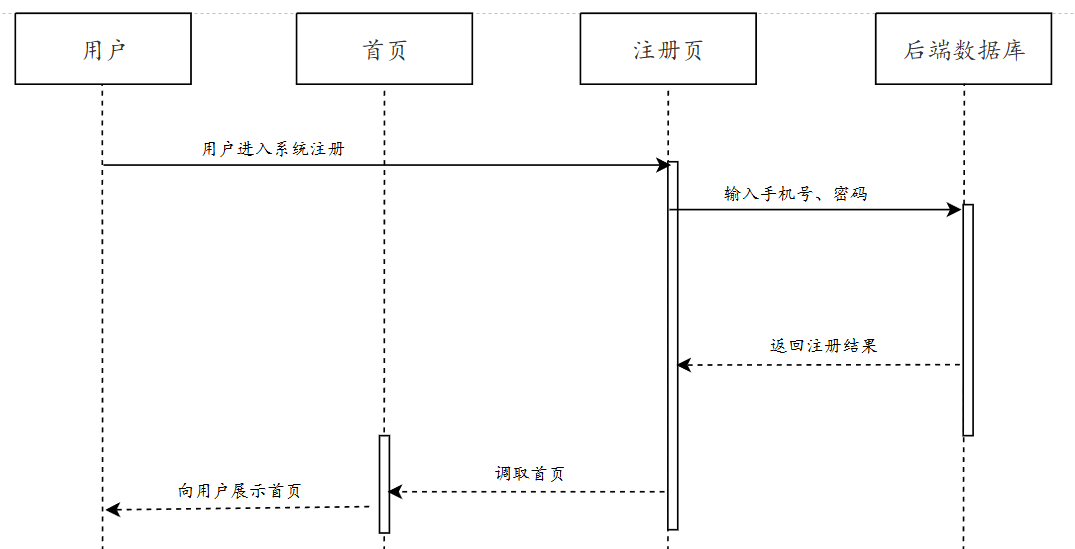
\includegraphics[width=0.7\textwidth]{figures/use321.png}
\end{figure}

\noindent\textbf{用例}

\begin{xltabular}{\linewidth}{|>{\raggedright\arraybackslash}p{3cm}|>{\raggedright\arraybackslash}p{8cm}|}
  \hline
  \textbf{用例} & 注册 \\ \hline 
  \endfirsthead
  
  \hline
  \textbf{用例} & 注册 (续) \\ \hline 
  \endhead
  
  \hline
  \multicolumn{2}{r}{接下页} \\ 
  \endfoot
  
  \hline 
  \endlastfoot
  
  \textbf{主要参与者} & 普通用户/管理员 \\ \hline
  \textbf{目标} & 完成用户注册 \\ \hline
  \textbf{前提条件} & 无 \\ \hline
  \textbf{工作流程} & 
  \vspace{-0.5em}
  \begin{itemize}[topsep=0pt, partopsep=0pt, left=0pt, nosep]
    \item 用户点击界面的注册按钮
    \item 系统跳转到注册界面
    \item 用户输入手机号和账号密码
    \item 系统验证后跳转首页
  \end{itemize} \\ \hline
  \textbf{触发器} & 系统用户需要使用系统 \\ \hline
  \textbf{异常} & 
  \vspace{-0.5em}
  \begin{itemize}[topsep=0pt, partopsep=0pt, left=0pt, nosep]
    \item 首页无法跳转至注册页面
    \item 已有账号的手机号无法注册
    \item 注册界面无法跳转至首页
    \item 浏览器弹出一个错误页面
  \end{itemize} \\ \hline
  \textbf{优先级} & 必须实现 \\ \hline
  \textbf{使用频率} & 频繁 \\ \hline
  \textbf{使用方式} & 通过浏览器 \\ \hline
  \textbf{次要参与者} & 无 \\ \hline
\end{xltabular}



\subsubsection{用户登录}

\noindent\textbf{描述及优先级}

用户和管理员在使用此动物领养系统时必须首先登录自己注册的账号。登录方式采用手机号或账号和密码登录。系统将根据登录账号信息返回不同的内容,如普通用户的首页和管理员的首页。

优先级:极高(系统基础功能,必须实现)

\noindent\textbf{主要流程请求/响应时序图}

\begin{figure}[H]
  \centering
  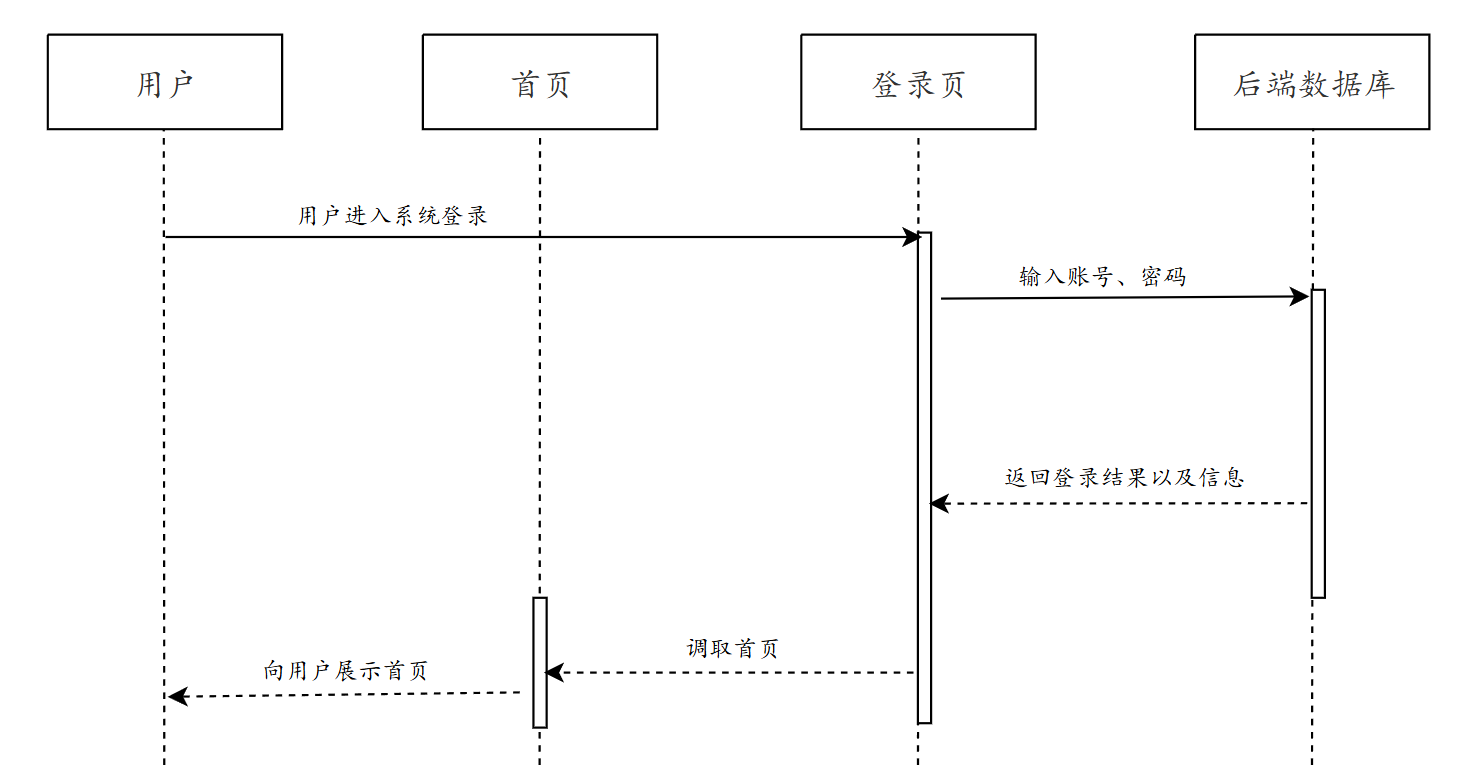
\includegraphics[width=0.7\textwidth]{figures/use322.png}
\end{figure}

\noindent\textbf{用例}

\begin{xltabular}{\linewidth}{|>{\raggedright\arraybackslash}p{3cm}|>{\raggedright\arraybackslash}p{8cm}|}
  \hline
  \textbf{用例} & 登录 \\ \hline 
  \endfirsthead
  
  \hline
  \textbf{用例} & 登录 (续) \\ \hline 
  \endhead
  
  \hline
  \multicolumn{2}{r}{续下页} \\ 
  \endfoot

  \hline \endlastfoot

  \textbf{主要参与者} & 普通用户/管理员 \\ \hline
  \textbf{目标} & 完成用户登录 \\ \hline
  \textbf{前提条件} & 用户已有个人账号 \\ \hline
  \textbf{工作流程} & 
  \vspace{-0.5em}
  \begin{itemize}[topsep=0pt, partopsep=0pt, left=0pt, nosep]
      \item 用户点击界面的 登录 按钮
      \item 系统跳转到登录界面
      \item 用户输入账号密码
      \item 系统验证后跳转首页
  \end{itemize} \\ \hline
  \textbf{拓展点} &
  \vspace{-0.5em}
  \begin{itemize}[topsep=0pt, partopsep=0pt, left=0pt, nosep]
      \item 提供忘记密码功能,可以找回账号
      \item 记录显示上次登陆时间
  \end{itemize} \\ \hline
  \textbf{触发器} & 系统用户需要使用系统 \\ \hline
  \textbf{异常} & 
  \vspace{-0.5em}
  \begin{itemize}[topsep=0pt, partopsep=0pt, left=0pt, nosep]
      \item 首页无法跳转至登录页面
      \item 账号密码错误
      \item 注册界面无法跳转至首页
      \item 浏览器弹出一个错误页面
  \end{itemize} \\ \hline
  \textbf{优先级} & 必须实现 \\ \hline
  \textbf{使用频率} & 非常频繁 \\ \hline
  \textbf{使用方式} & 通过浏览器 \\ \hline
  \textbf{次要参与者} & 无 \\ \hline
\end{xltabular}

\subsubsection{个人信息}

\noindent\textbf{描述及优先级}

用户在使用系统的过程中,可以随时查看和修改自己的个人信息,包括自己的昵称、性别、年龄、手机号和地址等信息。

优先级:高(系统基础功能,必须实现)

\noindent\textbf{主要流程请求/响应时序图}

\begin{figure}[H]
  \centering
  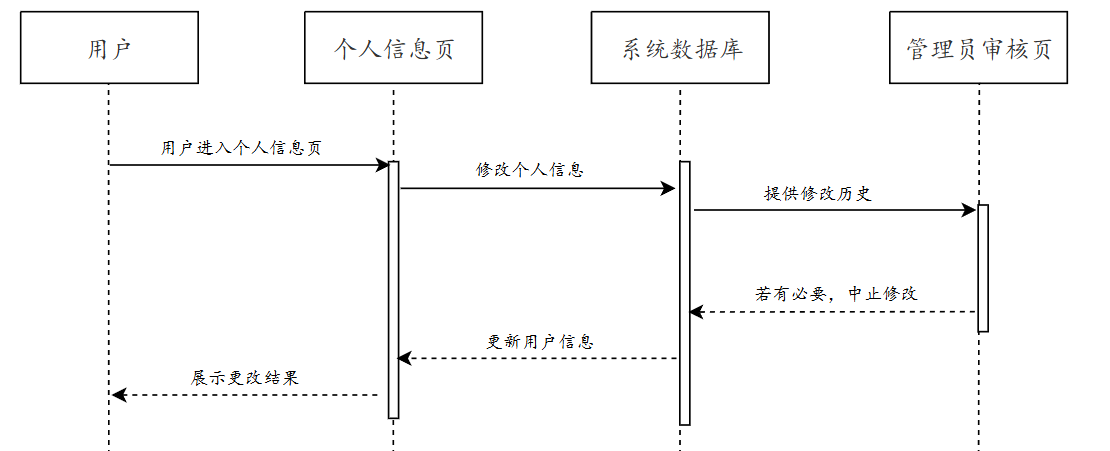
\includegraphics[width=0.7\textwidth]{figures/use323.png}
\end{figure}

\noindent\textbf{用例}

\begin{xltabular}{\linewidth}{|>{\raggedright\arraybackslash}p{3cm}|>{\raggedright\arraybackslash}p{8cm}|}
  \hline
  \textbf{用例} & 个人信息 \\ \hline \endfirsthead
  \hline
  \textbf{用例} & 个人信息 \\ \hline \endhead
  \hline
  \multicolumn{2}{r}{续下页} \\ \endfoot
  \hline \endlastfoot

  \textbf{主要参与者} & 普通用户/管理员 \\ \hline
  \textbf{目标} & 用户可自由修改个人信息 \\ \hline
  \textbf{前提条件} & 用户完成登录 \\ \hline
  \textbf{工作流程} & 
  \vspace{-0.5em}
  \begin{itemize}[topsep=0pt, partopsep=0pt, left=0pt, nosep]
      \item 用户点击个人信息页的修改
      \item 系统记录用户修改的内容
      \item 系统自动审核并提交管理员
      \item 完成修改,返回个人信息页
      \item 系统提示修改结果
  \end{itemize} \\ \hline
  \textbf{拓展点} &
  \vspace{-0.5em}
  \begin{itemize}[topsep=0pt, partopsep=0pt, left=0pt, nosep]
      \item 管理员可以查看和拒绝修改
      \item 允许设置个人资料隐私权限
      \item 显示个人活动记录
  \end{itemize} \\ \hline
  \textbf{触发器} & 系统用户需要进行个人信息修改 \\ \hline
  \textbf{异常} & 
  \vspace{-0.5em}
  \begin{itemize}[topsep=0pt, partopsep=0pt, left=0pt, nosep]
      \item 修改按钮无响应
      \item 系统无法记录用户修改的内容
      \item 系统无法返回修改结果
      \item 系统无法判断修改合理性
  \end{itemize} \\ \hline
  \textbf{优先级} & 必须实现 \\ \hline
  \textbf{使用频率} & 频繁 \\ \hline
  \textbf{使用方式} & 通过浏览器 \\ \hline
  \textbf{次要参与者} & 无 \\ \hline
\end{xltabular}

\subsubsection{动物详细信息}

\noindent\textbf{描述及优先级}

在动物领养系统中一个重要点就是用户可以自由查看需要领养的流浪动物详尽信息,从中了解动物的基本信息、健康状况、性格特点、领养要求等。用户可以通过动物的照片和详细信息来判断是否适合领养该动物。并且也能由用户创建新的动物信息和新建新动物。管理员可以审核用户创建的动物信息,确保信息的真实性和准确性。

优先级:极高(系统基础功能,必须实现)

\noindent\textbf{主要流程请求/响应时序图}

\begin{figure}[H]
  \centering
  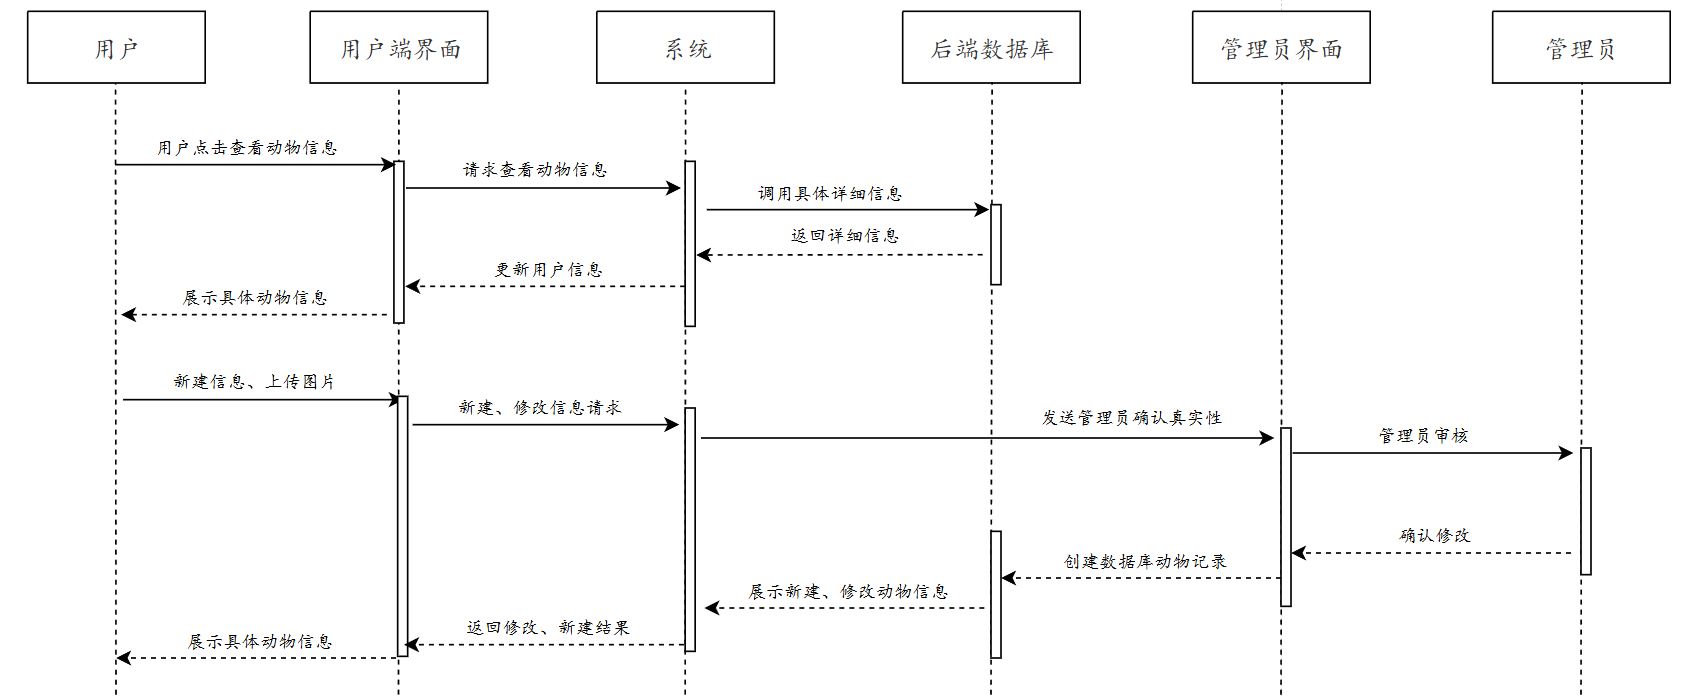
\includegraphics[width=0.8\textwidth]{figures/use324.png}
\end{figure}

\noindent\textbf{用例}

\begin{xltabular}{\linewidth}{|>{\raggedright\arraybackslash}p{3cm}|>{\raggedright\arraybackslash}p{8cm}|}
  \hline
  \textbf{用例} & 动物详细信息 \\ \hline \endfirsthead
  \hline
  \textbf{用例} & 动物详细信息 \\ \hline \endhead
  \hline
  \multicolumn{2}{r}{续下页} \\ \endfoot
  \hline \endlastfoot

  \textbf{主要参与者} & 普通用户/管理员 \\ \hline
  \textbf{目标} & 用户可查看、新建、修改动物信息 \\ \hline
  \textbf{前提条件} & 用户完成登录 \\ \hline
  \textbf{工作流程} & 
  \vspace{-0.5em}
  \begin{itemize}[topsep=0pt, partopsep=0pt, left=0pt, nosep]
      \item 用户点击查看某个动物详细信息
      \item 系统返回该动物详细信息
      \item 用户进行新建、修改动物信息或上传照片等
      \item 系统记录用户修改内容,发送管理员审核
      \item 管理员完成审核,数据库更新
      \item 返回更新后的动物信息
  \end{itemize} \\ \hline
  \textbf{拓展点} &
  \vspace{-0.5em}
  \begin{itemize}[topsep=0pt, partopsep=0pt, left=0pt, nosep]
      \item 支持上传动物视频
      \item 增加收藏功能,方便用户追踪
      \item 提供分享功能
  \end{itemize} \\ \hline
  \textbf{触发器} & 用户点击、新建、上传动物信息 \\ \hline
  \textbf{异常} & 
  \vspace{-0.5em}
  \begin{itemize}[topsep=0pt, partopsep=0pt, left=0pt, nosep]
      \item 系统功能无响应
      \item 动物信息未同步显示在数据库和用户界面
      \item 系统无法记录用户修改的内容
      \item 管理员无法审核修改的内容
  \end{itemize} \\ \hline
  \textbf{优先级} & 必须实现 \\ \hline
  \textbf{使用频率} & 非常频繁 \\ \hline
  \textbf{使用方式} & 通过浏览器 \\ \hline
  \textbf{次要参与者} & 无 \\ \hline
\end{xltabular}

\subsubsection{动物领养申请与审批}

\noindent\textbf{描述及优先级}

此功能是动物领养系统的核心功能。管理员可以发布动物的领养信息,供用户查看和申请。用户可以通过系统提交领养申请,然后由管理员进行领养条件审核,完成领养申请的审批,更新动物的领养状态,通知用户领养结果。

优先级:极高(系统基础功能,必须实现)

\noindent\textbf{主要流程请求/响应时序图}

\begin{figure}[H]
  \centering
  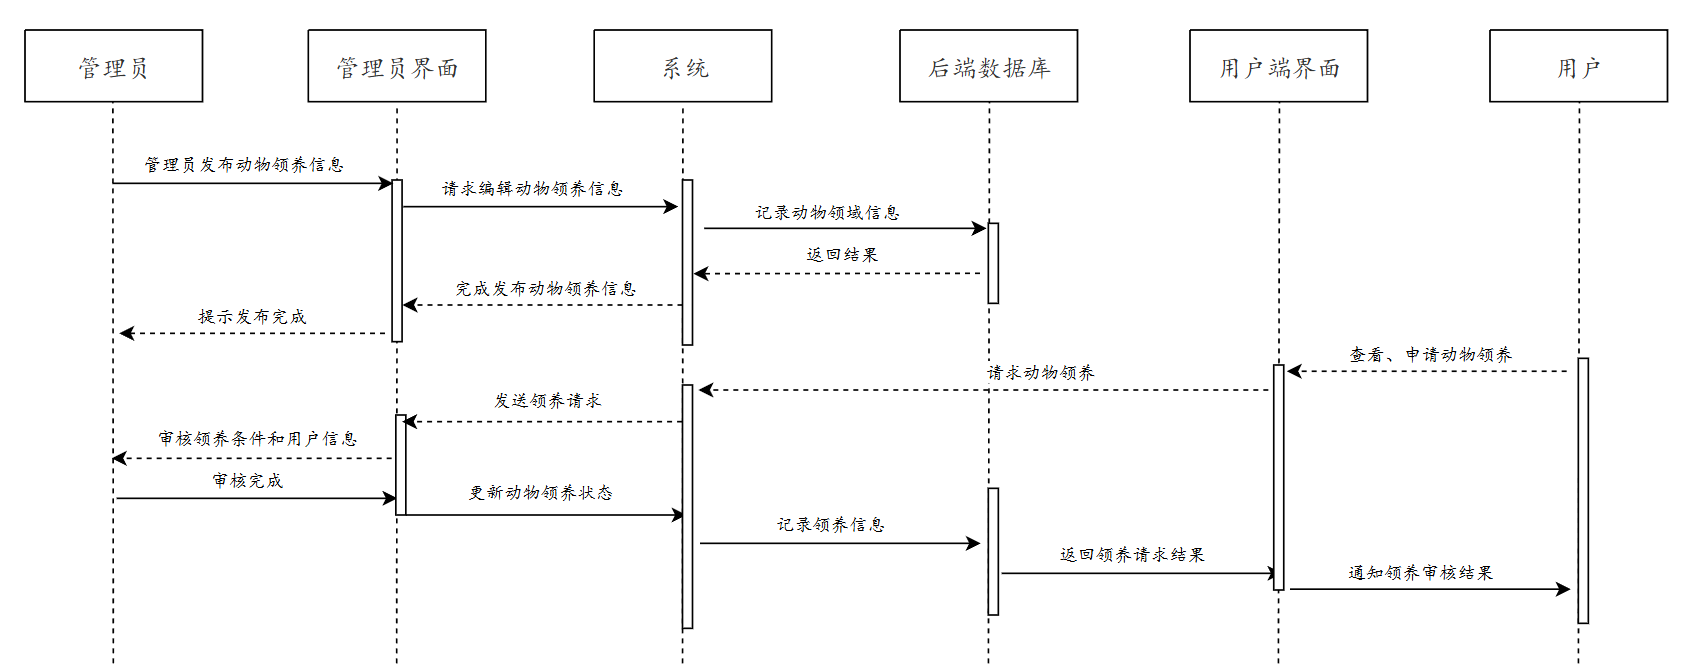
\includegraphics[width=0.8\textwidth]{figures/use325.png} 
\end{figure}

\noindent\textbf{用例}

\begin{xltabular}{\linewidth}{|>{\raggedright\arraybackslash}p{3cm}|>{\raggedright\arraybackslash}p{8cm}|}
  \hline
  \textbf{用例} & 动物领养 \\ \hline \endfirsthead
  \hline
  \textbf{用例} & 动物领养 \\ \hline \endhead
  \hline
  \multicolumn{2}{r}{续下页} \\ \endfoot
  \hline \endlastfoot

  \textbf{主要参与者} & 普通用户/管理员 \\ \hline
  \textbf{目标} & 用户可申请领养,管理员可发布和审核领养 \\ \hline
  \textbf{前提条件} & 用户完成登录与领养条件登记 \\ \hline
  \textbf{工作流程} & 
  \vspace{-0.5em}
  \begin{itemize}[topsep=0pt, partopsep=0pt, left=0pt, nosep]
      \item 管理员发布新的动物领养信息
      \item 系统更新动物领养信息,供用户查看
      \item 用户点击申请领养,发送申请信息
      \item 管理员审核用户的领养申请
      \item 系统更新领养状态,通知申请用户审核结果
  \end{itemize} \\ \hline
  \textbf{拓展点} &
  \vspace{-0.5em}
  \begin{itemize}[topsep=0pt, partopsep=0pt, left=0pt, nosep]
      \item 设计标准化的在线领养申请表单
      \item 用户可以实时追踪申请状态
      \item 增加申请者和管理员的站内沟通功能
      \item 允许用户撤销自己的申请
  \end{itemize} \\ \hline
  \textbf{触发器} & 用户点击、新建、上传动物信息 \\ \hline
  \textbf{异常} & 
  \vspace{-0.5em}
  \begin{itemize}[topsep=0pt, partopsep=0pt, left=0pt, nosep]
      \item 系统功能无响应
      \item 领养信息无法发布,无法查看
      \item 领养状态未同步
      \item 管理员无法审核领养申请
  \end{itemize} \\ \hline
  \textbf{优先级} & 必须实现 \\ \hline
  \textbf{使用频率} & 频繁 \\ \hline
  \textbf{使用方式} & 通过浏览器 \\ \hline
  \textbf{次要参与者} & 无 \\ \hline
\end{xltabular}

\subsubsection{动物领养指南}

\noindent\textbf{描述及优先级}

动物领养指南是一个重要的功能模块,用户可以在系统中查看和学习动物领养的相关知识和技巧。管理员可以发布和更新领养指南,确保用户获取最新的信息和建议。通过发布和更新领养指南,管理员可以帮助用户更好地了解领养动物的注意事项和技巧,提高领养成功率。

优先级:高(系统基础功能,必须实现)

\noindent\textbf{主要流程请求/响应时序图}

\begin{figure}[H]
  \centering
  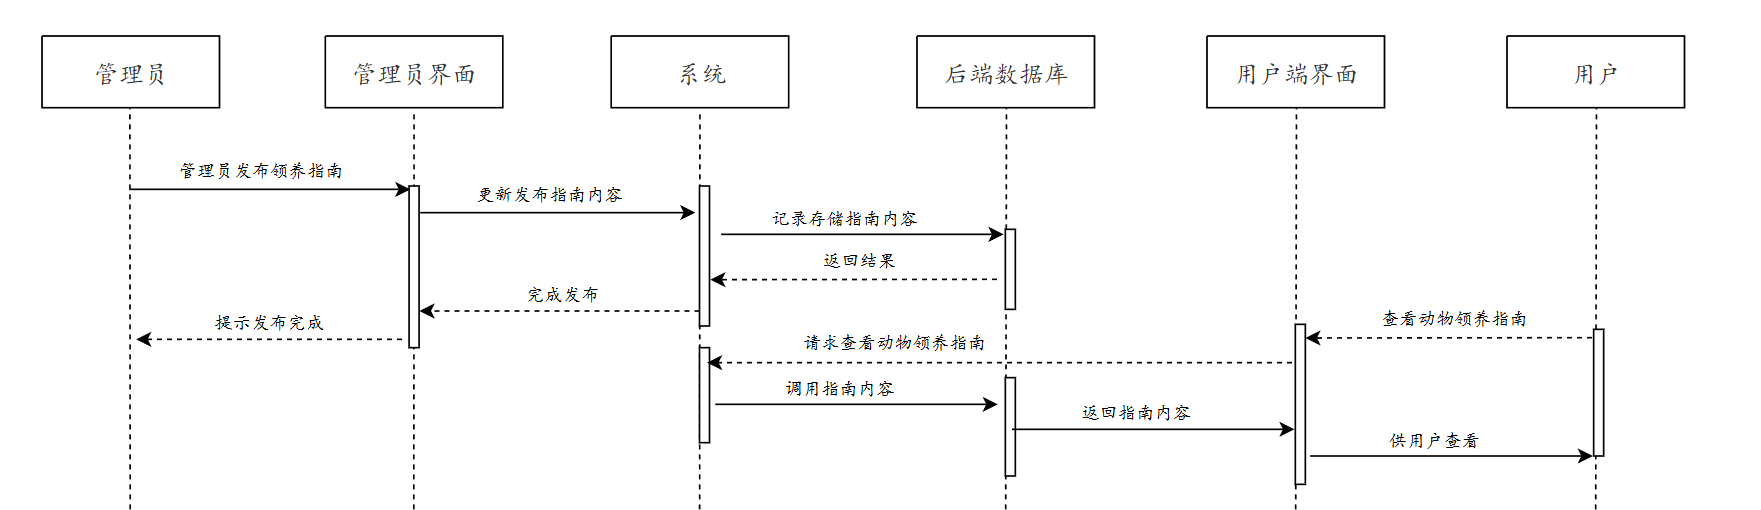
\includegraphics[width=0.8\textwidth]{figures/use326.png} 
\end{figure}

\noindent\textbf{用例}

\begin{xltabular}{\linewidth}{|>{\raggedright\arraybackslash}p{3cm}|>{\raggedright\arraybackslash}p{8cm}|}
  \hline
  \textbf{用例} & 动物指南 \\ \hline \endfirsthead
  \hline
  \textbf{用例} & 动物指南 \\ \hline \endhead
  \hline
  \multicolumn{2}{r}{续下页} \\ \endfoot
  \hline \endlastfoot

  \textbf{主要参与者} & 普通用户/管理员 \\ \hline
  \textbf{目标} & 用户可学习领养指南 \\ \hline
  \textbf{前提条件} & 用户完成登录 \\ \hline
  \textbf{工作流程} & 
  \vspace{-0.5em}
  \begin{itemize}[topsep=0pt, partopsep=0pt, left=0pt, nosep]
      \item 管理员发布动物领养指南
      \item 系统更新动物领养指南
      \item 用户点击查看领养指南
      \item 系统返回领养指南
  \end{itemize} \\ \hline
  \textbf{拓展点} &
  \vspace{-0.5em}
  \begin{itemize}[topsep=0pt, partopsep=0pt, left=0pt, nosep]
      \item 可以提供全网搜索指南内容
  \end{itemize} \\ \hline
  \textbf{触发器} & 用户点击、新建、上传动物信息 \\ \hline
  \textbf{异常} & 
  \vspace{-0.5em}
  \begin{itemize}[topsep=0pt, partopsep=0pt, left=0pt, nosep]
      \item 系统功能无响应
      \item 领养指南无法发布,无法查看
      \item 用户无法查看领养指南
  \end{itemize} \\ \hline
  \textbf{优先级} & 必须实现 \\ \hline
  \textbf{使用频率} & 频繁 \\ \hline
  \textbf{使用方式} & 通过浏览器 \\ \hline
  \textbf{次要参与者} & 无 \\ \hline
\end{xltabular}

\subsubsection{动物地图}

\noindent\textbf{描述及优先级}

用户可以通过查看地图来了解动物的分布情况和位置,以此更能了解动物的具体情况。用户也可以选择更新某个动物的实时位置。

优先级:高(系统基础功能,必须实现)

\noindent\textbf{主要流程请求/响应时序图}

\begin{figure}[H]
  \centering
  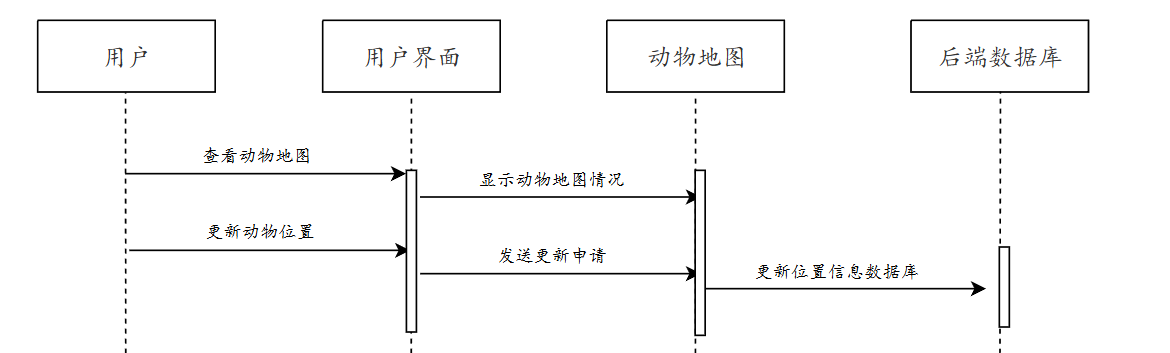
\includegraphics[width=0.8\textwidth]{figures/use327.png}
\end{figure}

\noindent\textbf{用例}

\begin{xltabular}{\linewidth}{|>{\raggedright\arraybackslash}p{3cm}|>{\raggedright\arraybackslash}p{8cm}|}
  \hline
  \textbf{用例} & 动物地图 \\ \hline \endfirsthead
  \hline
  \textbf{用例} & 动物地图 \\ \hline \endhead
  \hline
  \multicolumn{2}{r}{续下页} \\ \endfoot
  \hline \endlastfoot

  \textbf{主要参与者} & 用户 \\ \hline
  \textbf{目标} & 用户可使用动物定位地图 \\ \hline
  \textbf{前提条件} & 用户完成登录 \\ \hline
  \textbf{工作流程} & 
  \vspace{-0.5em}
  \begin{itemize}[topsep=0pt, partopsep=0pt, left=0pt, nosep]
      \item 用户查看动物地图
      \item 系统返回动物地图信息
      \item 用户更新某动物定位
      \item 系统修改定位数据
  \end{itemize} \\ \hline
  \textbf{拓展点} &
  \vspace{-0.5em}
  \begin{itemize}[topsep=0pt, partopsep=0pt, left=0pt, nosep]
      \item 提供更丰富的地图样式
      \item 提供动物定位的历史记录
  \end{itemize} \\ \hline
  \textbf{触发器} & 用户点击、新建、上传动物信息 \\ \hline
  \textbf{异常} & 
  \vspace{-0.5em}
  \begin{itemize}[topsep=0pt, partopsep=0pt, left=0pt, nosep]
      \item 系统功能无响应
      \item 动物地图无法查看
      \item 用户无法修改动物定位
  \end{itemize} \\ \hline
  \textbf{优先级} & 应该实现 \\ \hline
  \textbf{使用频率} & 频繁 \\ \hline
  \textbf{使用方式} & 通过浏览器 \\ \hline
  \textbf{次要参与者} & 无 \\ \hline
\end{xltabular}

\subsubsection{动物识图}

\noindent\textbf{描述及优先级}

用户可能会在校园和其他位置看见一些已经有信息的动物,但不知道动物的具体信息。用户可以通过拍照或上传图片的方式来识别动物,系统会自动识别动物的种类和信息,并返回给用户。

优先级:高(系统基础功能,必须实现)

\noindent\textbf{主要流程请求/响应时序图}

\begin{figure}[H]
  \centering
  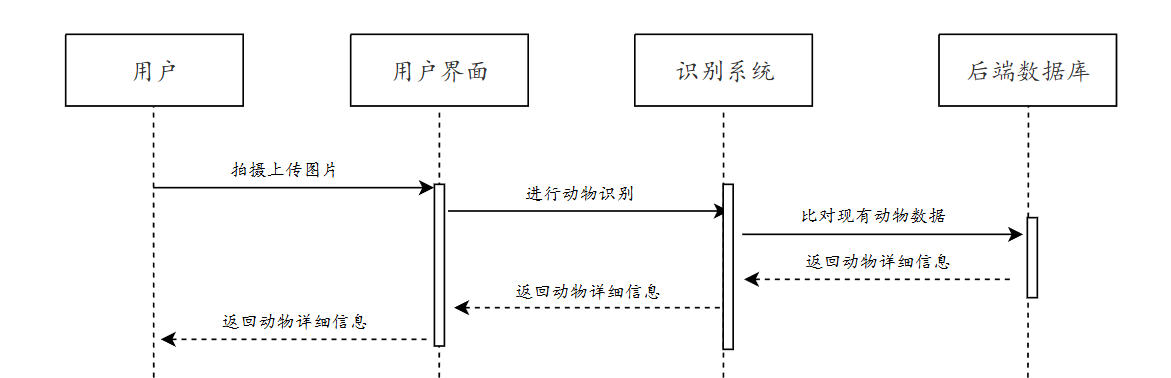
\includegraphics[width=0.8\textwidth]{figures/use328.png}
\end{figure}  

\noindent\textbf{用例}

\begin{xltabular}{\linewidth}{|>{\raggedright\arraybackslash}p{3cm}|>{\raggedright\arraybackslash}p{8cm}|}
  \hline
  \textbf{用例} & 动物识别 \\ \hline \endfirsthead
  \hline
  \textbf{用例} & 动物识别 \\ \hline \endhead
  \hline
  \multicolumn{2}{r}{续下页} \\ \endfoot
  \hline \endlastfoot

  \textbf{主要参与者} & 用户 \\ \hline
  \textbf{目标} & 用户可使用识别功能 \\ \hline
  \textbf{前提条件} & 用户完成登录 \\ \hline
  \textbf{工作流程} & 
  \vspace{-0.5em}
  \begin{itemize}[topsep=0pt, partopsep=0pt, left=0pt, nosep]
      \item 用户拍摄上传动物图片
      \item 系统识别动物信息
      \item 系统返回识别结果
  \end{itemize} \\ \hline
  \textbf{拓展点} &
  \vspace{-0.5em}
  \begin{itemize}[topsep=0pt, partopsep=0pt, left=0pt, nosep]
      \item 提供更丰富的识别功能
      \item 将此图片加入动物信息库
  \end{itemize} \\ \hline
  \textbf{触发器} & 用户点击动物识别搜索 \\ \hline
  \textbf{异常} & 
  \vspace{-0.5em}
  \begin{itemize}[topsep=0pt, partopsep=0pt, left=0pt, nosep]
      \item 系统功能无响应
      \item 动物识别无法查看
      \item 动物识别结果错误
  \end{itemize} \\ \hline
  \textbf{优先级} & 应该实现 \\ \hline
  \textbf{使用频率} & 频繁 \\ \hline
  \textbf{使用方式} & 通过浏览器 \\ \hline
  \textbf{次要参与者} & 无 \\ \hline
\end{xltabular}

\subsection{IPO 图}

\verb|IPO| 图是输入、处理和输出图,描述了系统的输入、处理和输出。它是一个重要的设计工具,可以帮助我们更好地理解系统的功能和数据流。

\subsubsection{用户端}

\begin{figure}[H]
  \centering
  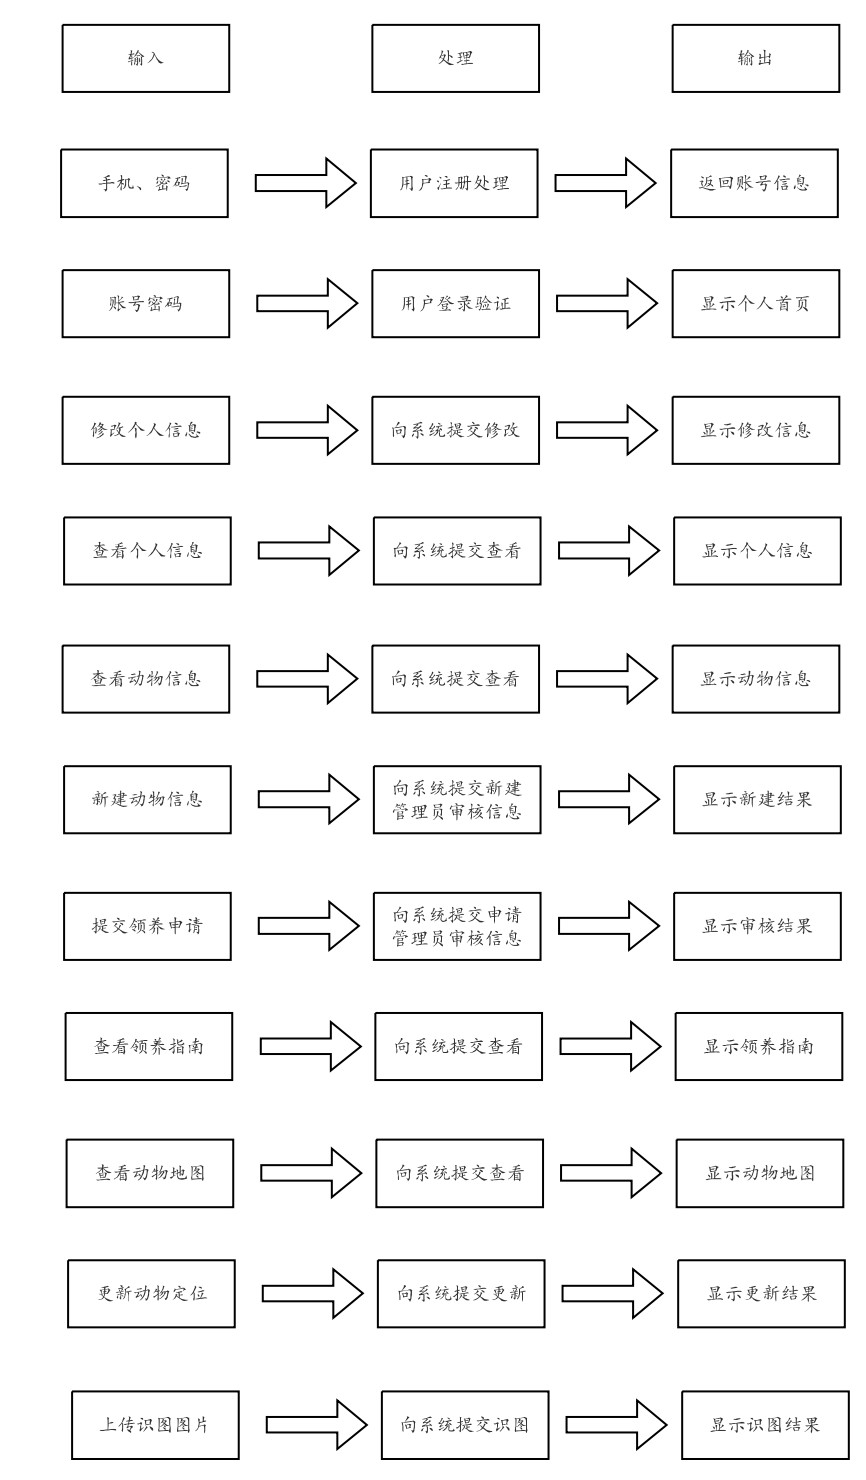
\includegraphics[width=0.8\textwidth]{figures/ipo1.png}
\end{figure}

\subsubsection{管理员端}

\begin{figure}[H]
  \centering
  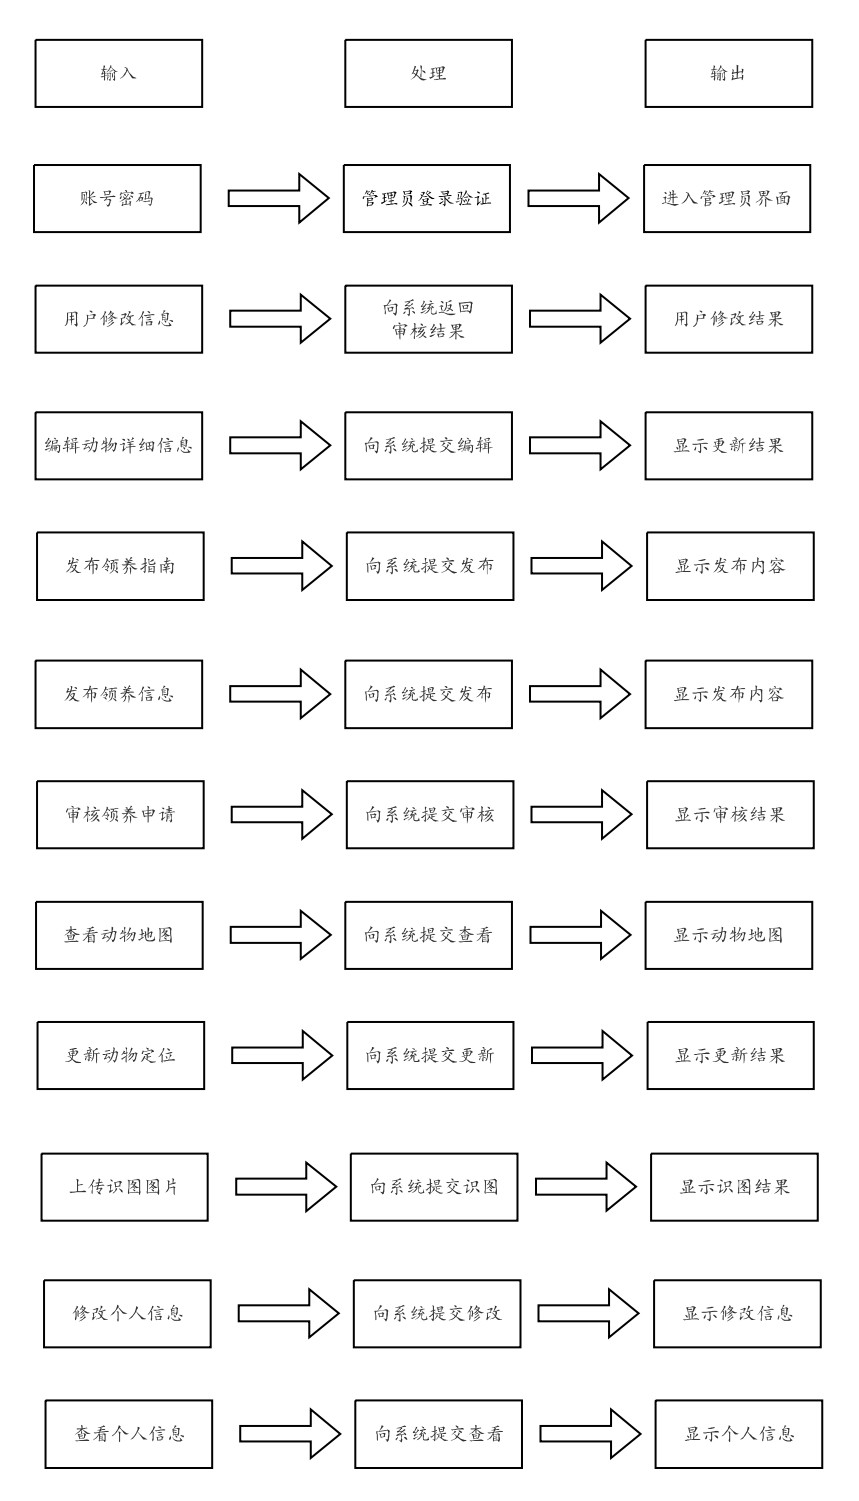
\includegraphics[width=0.8\textwidth]{figures/ipo2.png}
\end{figure}

\section{数据流图}

\subsection{顶层数据流图}

\begin{figure}[H]
  \centering
  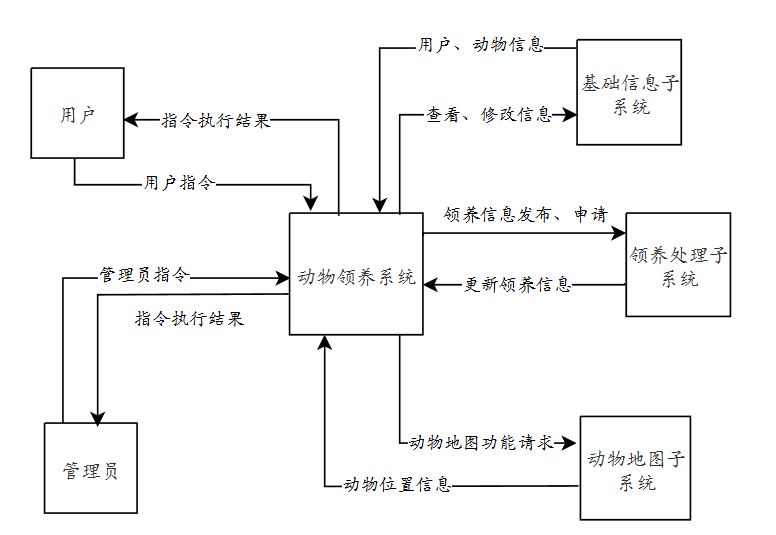
\includegraphics[width=0.7\textwidth]{figures/df1.png}
\end{figure}

\subsection{中层数据流图}

\begin{figure}[H]
  \centering
  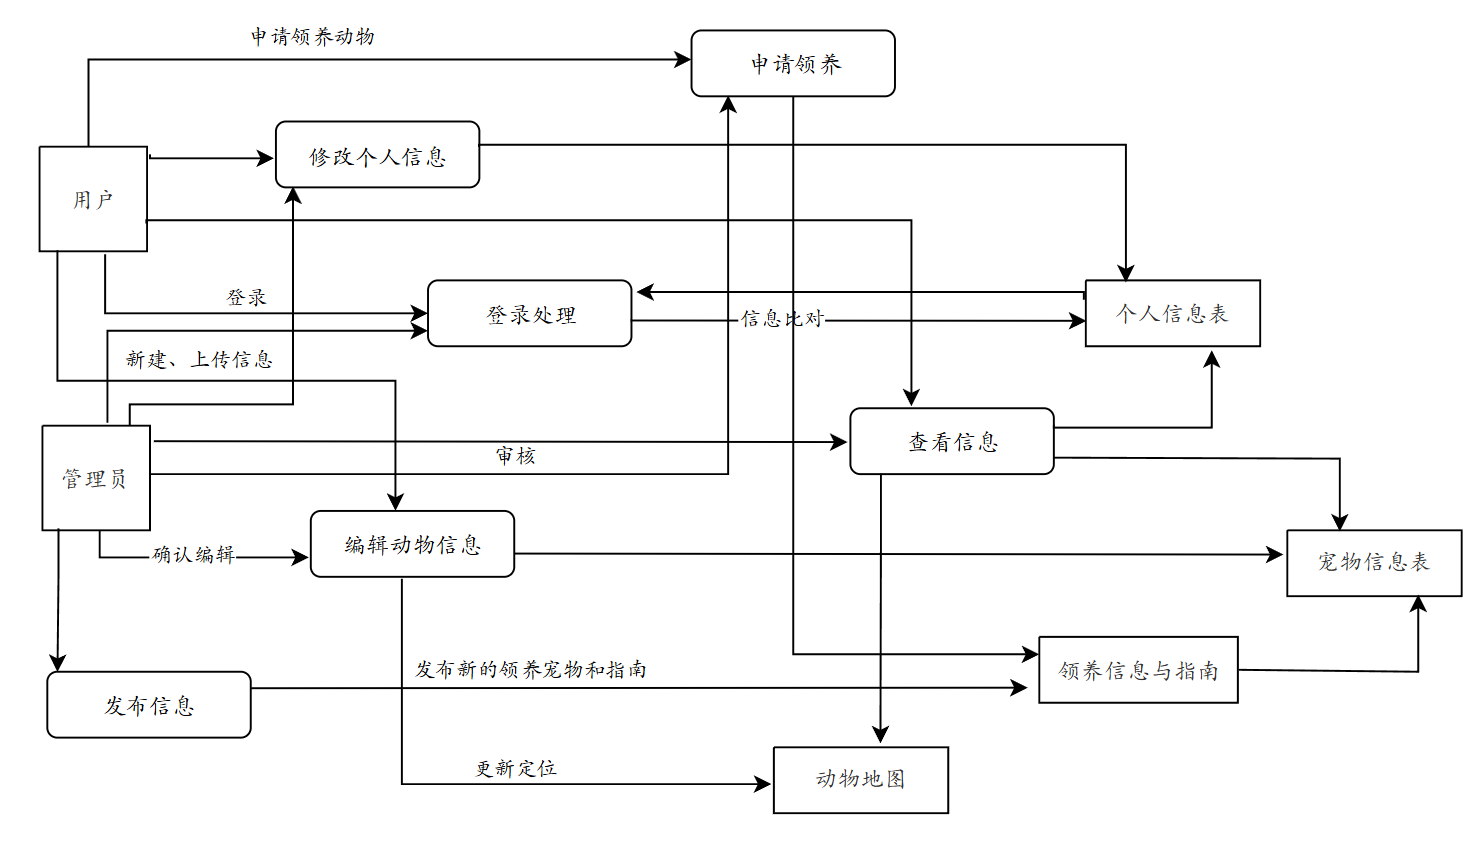
\includegraphics[width=0.9\textwidth]{figures/df2.png}
\end{figure}

\subsection{底层数据流图}

\subsubsection{登录处理}

\begin{figure}[H]
  \centering
  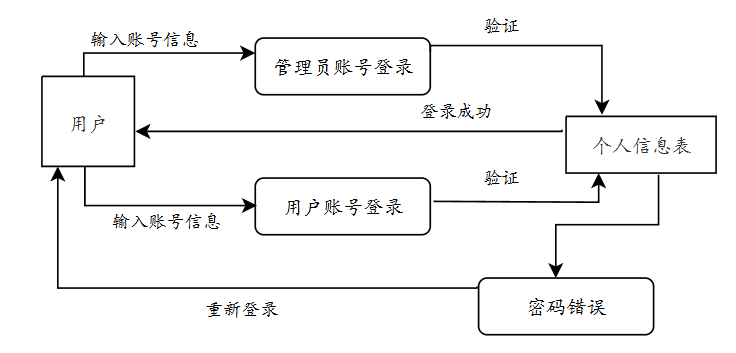
\includegraphics[width=0.65\textwidth]{figures/df31.png}
\end{figure}

\subsubsection{修改个人信息}

\begin{figure}[H]
  \centering
  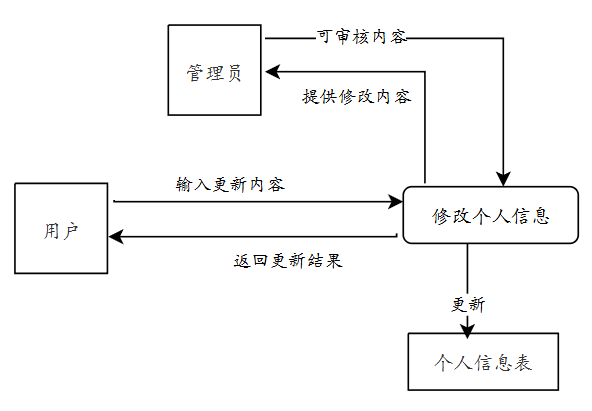
\includegraphics[width=0.5\textwidth]{figures/df32.png}
\end{figure}

\subsubsection{编辑动物信息}

\begin{figure}[H]
  \centering
  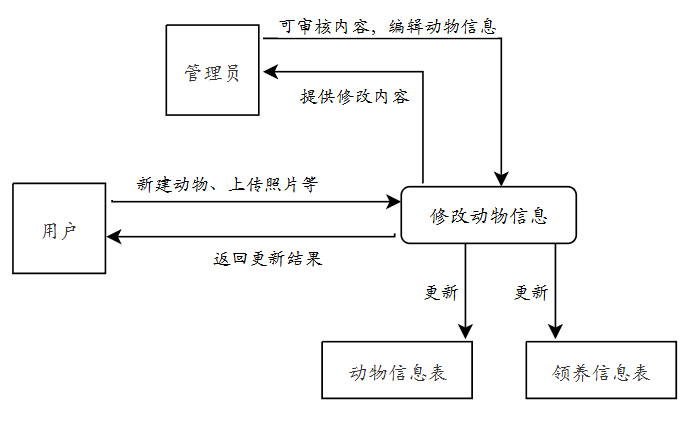
\includegraphics[width=0.5\textwidth]{figures/df33.png}
\end{figure}

\subsubsection{领养申请}

\begin{figure}[H]
  \centering
  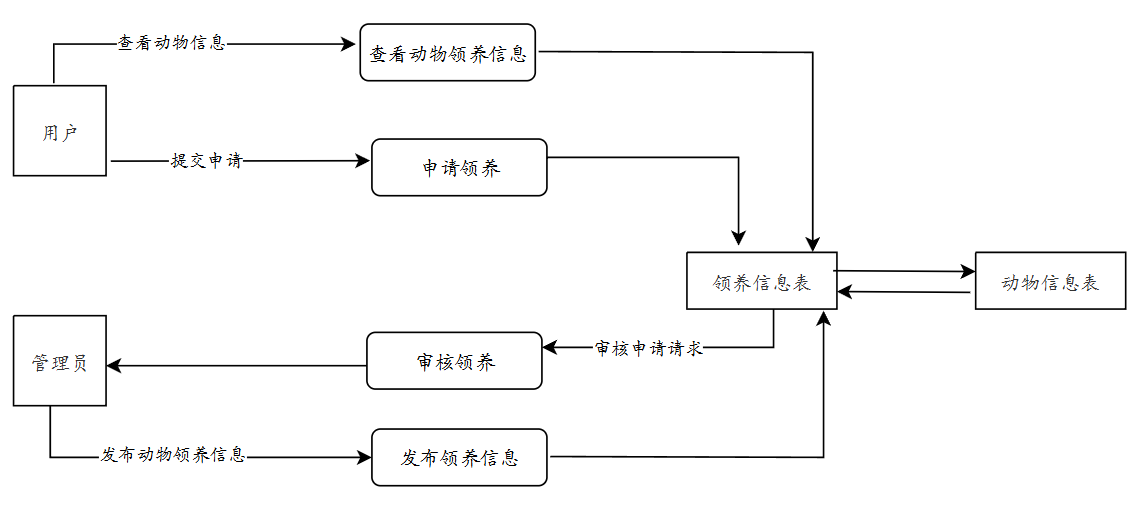
\includegraphics[width=0.8\textwidth]{figures/df34.png}
\end{figure}

\subsubsection{动物地图}

\begin{figure}[H]
  \centering
  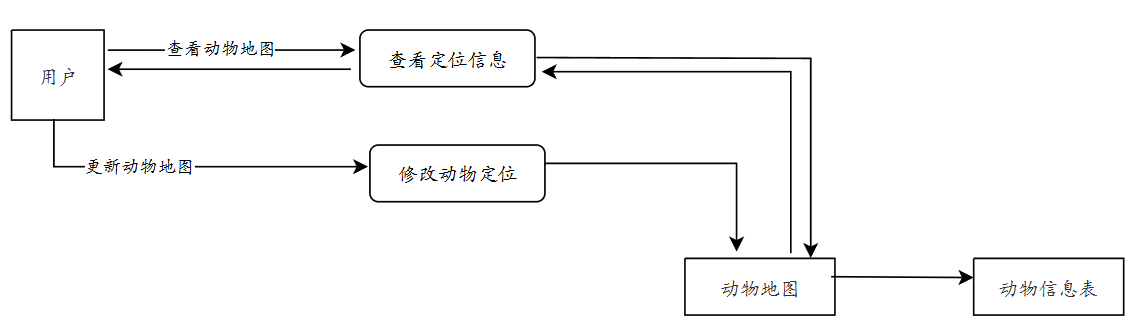
\includegraphics[width=0.8\textwidth]{figures/df35.png}
\end{figure}

\section{状态图}

\begin{figure}[H]
  \centering
  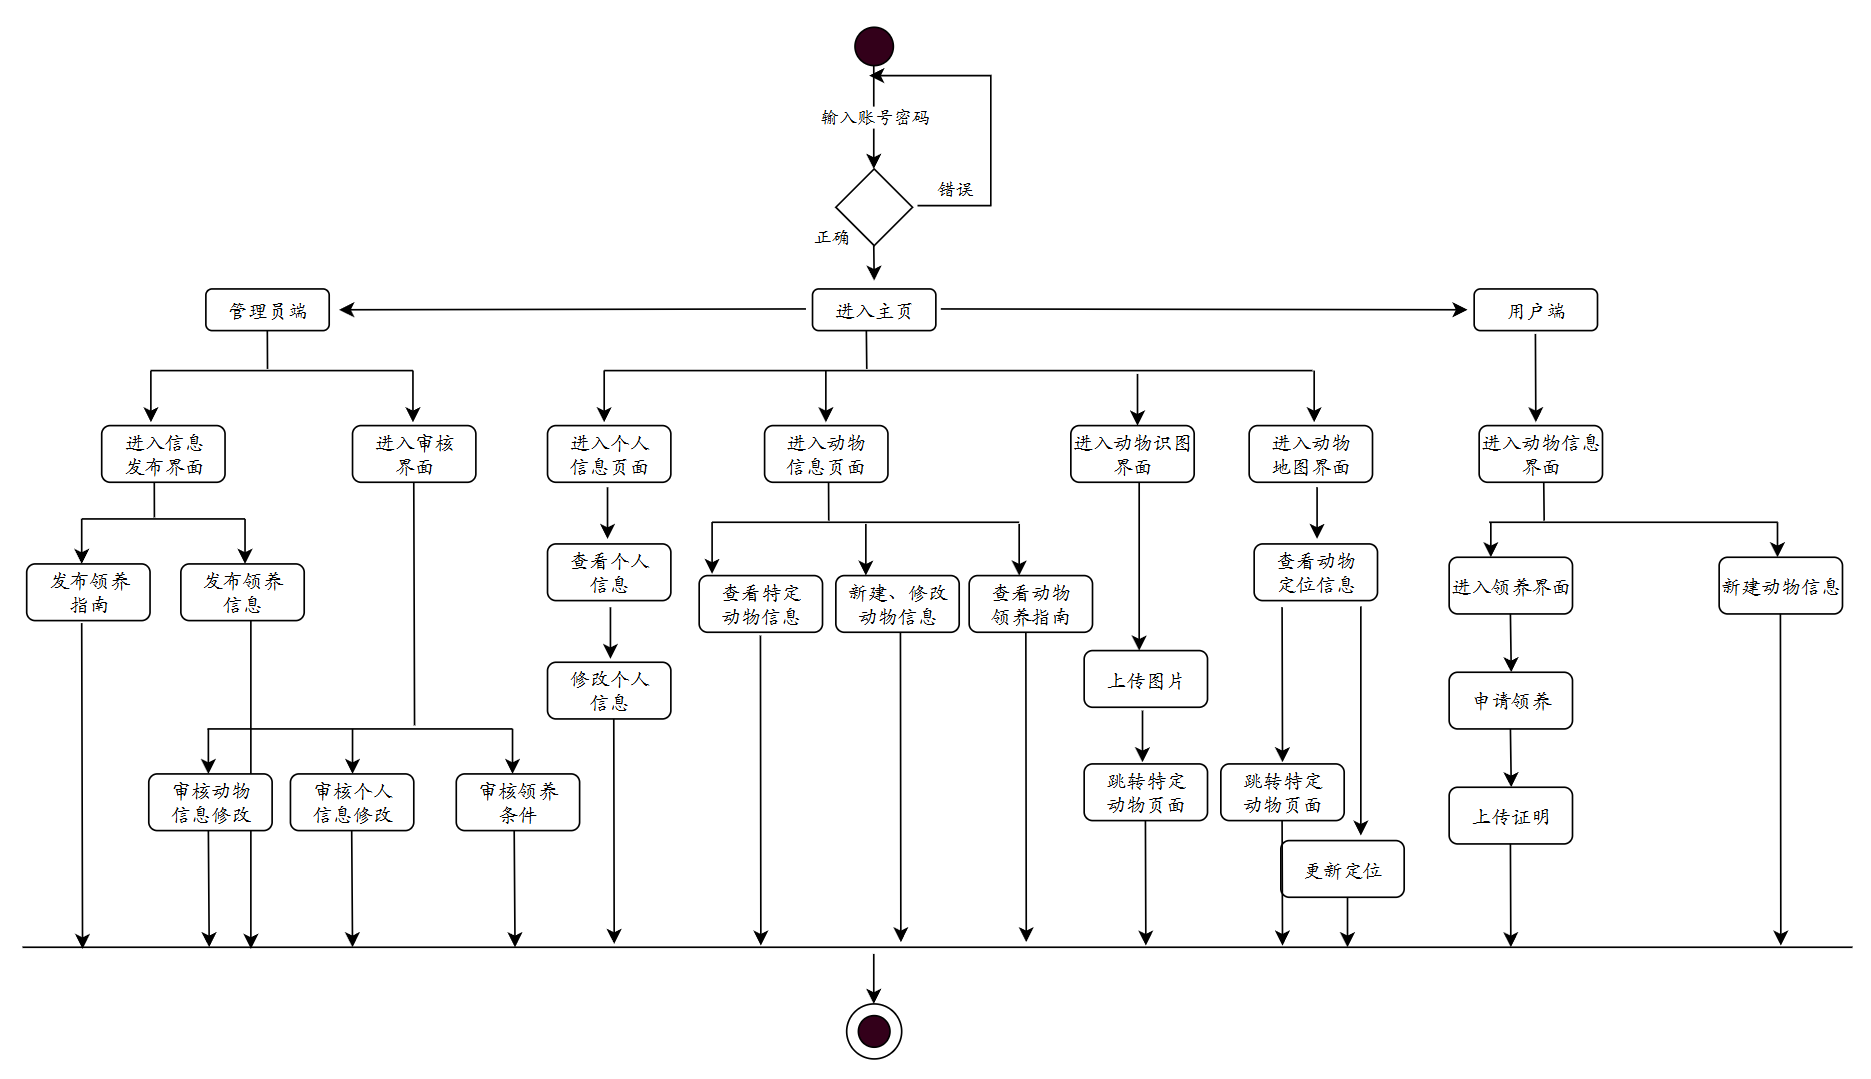
\includegraphics[width=0.98\textwidth]{figures/state.png}
\end{figure}

\section{CRC 卡}

\begin{xltabular}{\linewidth}{|>{\raggedright\arraybackslash}p{8cm}|>{\raggedright\arraybackslash}p{4cm}|}
  \hline
  \verb|Class| \textbf{普通用户} &  \\ \hline \endfirsthead
  \hline
  \verb|Class| \textbf{普通用户} &  \\ \hline \endhead
  \hline
  \multicolumn{2}{r}{续下页} \\ \endfoot
  \hline \endlastfoot

  \verb|RESPONSIBILITY| & \verb|COLLABORATOR| \\ \hline
  注册、登录、登出 & 个人信息 \\ \hline
  查看、修改个人信息 & 个人信息、管理员 \\ \hline
  查看、修改动物信息 & 动物、管理员 \\ \hline
  查看、更新动物地图 & 地图 \\ \hline
  提交领养申请 & 领养信息 \\ \hline
  使用动物识图 & 搜索识图 \\ \hline 
  查看领养指南 & 领养指南 \\ \hline
\end{xltabular}

\vspace{1cm}

\begin{xltabular}{\linewidth}{|>{\raggedright\arraybackslash}p{8cm}|>{\raggedright\arraybackslash}p{4cm}|}
  \hline
  \verb|Class| \textbf{管理员} &  \\ \hline \endfirsthead
  \hline
  \verb|Class| \textbf{管理员} &  \\ \hline \endhead
  \hline
  \multicolumn{2}{r}{续下页} \\ \endfoot
  \hline \endlastfoot

  \verb|RESPONSIBILITY| & \verb|COLLABORATOR| \\ \hline
  登录、登出 & 个人信息 \\ \hline
  审核用户个人信息修改 & 个人信息 \\ \hline
  查看编辑动物信息 & 动物 \\ \hline
  发布、审核领养申请 & 领养信息、动物 \\ \hline
  使用动物识图 & 搜索识图 \\ \hline
  发布领养指南 & 领养指南 \\ \hline
  查看、更新动物地图 & 地图 \\ \hline
\end{xltabular}

\vspace{1cm}

\begin{xltabular}{\linewidth}{|>{\raggedright\arraybackslash}p{8cm}|>{\raggedright\arraybackslash}p{4cm}|}
  \hline
  \verb|Class| \textbf{动物} &  \\ \hline \endfirsthead
  \hline
  \verb|Class| \textbf{动物} &  \\ \hline \endhead
  \hline
  \multicolumn{2}{r}{续下页} \\ \endfoot
  \hline \endlastfoot

  \verb|RESPONSIBILITY| & \verb|COLLABORATOR| \\ \hline
  基本信息 (ID、名称、照片等) &  \\ \hline
  领养状态 & 领养信息 \\ \hline
  关联位置信息 & 地图 \\ \hline
  关联领养人 & 普通用户 \\ \hline
  关联负责管理员 & 管理员 \\ \hline
\end{xltabular}

\vspace{1cm}

\begin{xltabular}{\linewidth}{|>{\raggedright\arraybackslash}p{8cm}|>{\raggedright\arraybackslash}p{4cm}|}
  \hline
  \verb|Class| \textbf{个人信息} &  \\ \hline \endfirsthead
  \hline
  \verb|Class| \textbf{个人信息} &  \\ \hline \endhead
  \hline
  \multicolumn{2}{r}{续下页} \\ \endfoot
  \hline \endlastfoot

  \verb|RESPONSIBILITY| & \verb|COLLABORATOR| \\ \hline
  账户信息 & 普通用户、管理员 \\ \hline
  角色和状态 & 普通用户、管理员 \\ \hline
  领养情况证明 & 普通用户 \\ \hline
  领养关联 &  动物 \\ \hline
  审核情况 & 管理员 \\ \hline
\end{xltabular}

\vspace{1cm}

\begin{xltabular}{\linewidth}{|>{\raggedright\arraybackslash}p{8cm}|>{\raggedright\arraybackslash}p{4cm}|}
  \hline
  \verb|Class| \textbf{领养申请} &  \\ \hline \endfirsthead
  \hline
  \verb|Class| \textbf{领养申请} &  \\ \hline \endhead
  \hline
  \multicolumn{2}{r}{续下页} \\ \endfoot
  \hline \endlastfoot

  \verb|RESPONSIBILITY| & \verb|COLLABORATOR| \\ \hline
  申请状态 &  \\ \hline
  关联动物 & 动物 \\ \hline
  关联领养证明 & 个人信息 \\ \hline
  申请人 & 普通用户 \\ \hline
  审核人 &  管理员 \\ \hline
  审批状态 & 管理员 \\ \hline
\end{xltabular}

\vspace{1cm}

\begin{xltabular}{\linewidth}{|>{\raggedright\arraybackslash}p{8cm}|>{\raggedright\arraybackslash}p{4cm}|}
  \hline
  \verb|Class| \textbf{领养指南} &  \\ \hline \endfirsthead
  \hline
  \verb|Class| \textbf{领养指南} &  \\ \hline \endhead
  \hline
  \multicolumn{2}{r}{续下页} \\ \endfoot
  \hline \endlastfoot

  \verb|RESPONSIBILITY| & \verb|COLLABORATOR| \\ \hline
  指南内容 &  \\ \hline
  指南修改历史 & 管理员 \\ \hline
  指南涉及动物 & 动物 \\ \hline
  指南索引等 & \\ \hline
\end{xltabular}

\vspace{0.8cm}

\begin{xltabular}{\linewidth}{|>{\raggedright\arraybackslash}p{8cm}|>{\raggedright\arraybackslash}p{4cm}|}
  \hline
  \verb|Class| \textbf{地图} &  \\ \hline \endfirsthead
  \hline
  \verb|Class| \textbf{地图} &  \\ \hline \endhead
  \hline
  \multicolumn{2}{r}{续下页} \\ \endfoot
  \hline \endlastfoot

  \verb|RESPONSIBILITY| & \verb|COLLABORATOR| \\ \hline
  地图样式 &  \\ \hline
  提供位置查询 & 普通用户、管理员 \\ \hline
  动物地理位置和时间戳 & 动物 \\ \hline
  处理位置更新 &  普通用户、管理员 \\ \hline
\end{xltabular}

\vspace{1cm}

\begin{xltabular}{\linewidth}{|>{\raggedright\arraybackslash}p{8cm}|>{\raggedright\arraybackslash}p{4cm}|}
  \hline
  \verb|Class| \textbf{搜索识图} &  \\ \hline \endfirsthead
  \hline
  \verb|Class| \textbf{搜索识图} &  \\ \hline \endhead
  \hline
  \multicolumn{2}{r}{续下页} \\ \endfoot
  \hline \endlastfoot

  \verb|RESPONSIBILITY| & \verb|COLLABORATOR| \\ \hline
  动物图片库 & 动物 \\ \hline
  处理图片输入 & 普通用户 \\ \hline
  调用识别服务 &  \\ \hline
  匹配系统动物 & 动物 \\ \hline
\end{xltabular}

\section{类图}

\begin{figure}[H]
  \centering
  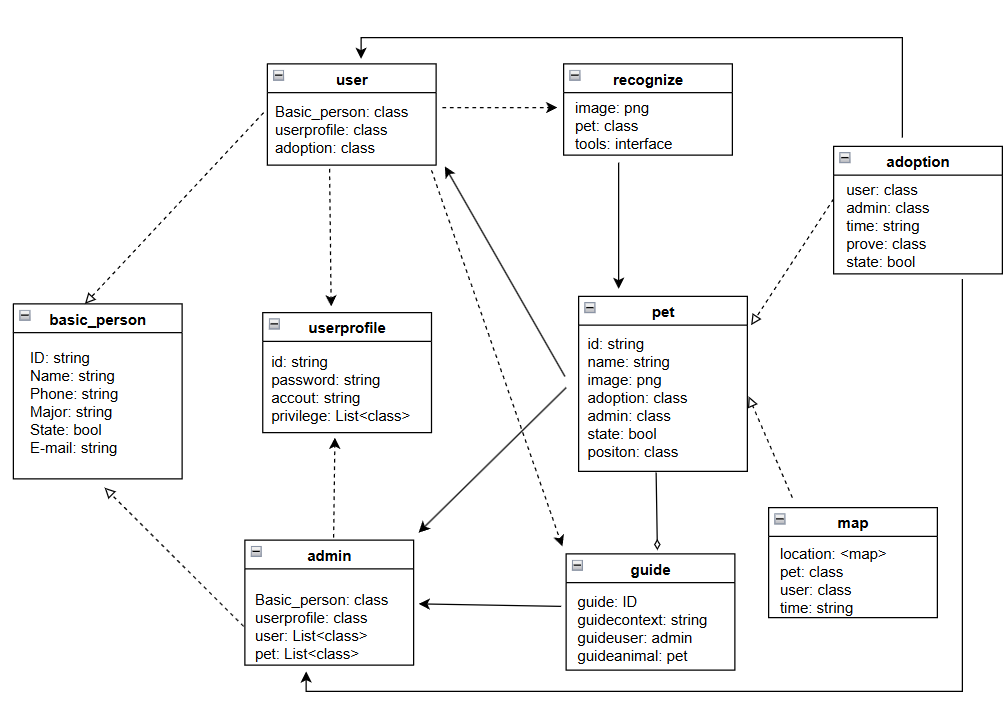
\includegraphics[width=0.8\textwidth]{figures/class.png}
\end{figure}

\section{数据词典}

\subsection{数据流定义表}

\renewcommand{\arraystretch}{1.45}

\begin{xltabular}{\linewidth}{
  |>{\centering\arraybackslash}m{1cm}
  |>{\centering\arraybackslash}m{3.5cm}
  |>{\centering\arraybackslash}m{3cm}
  |>{\centering\arraybackslash}m{3cm}
  |>{\centering\arraybackslash}m{5cm}|}
  \hline
  \textbf{编号} & \textbf{数据流名} & \textbf{来源} & \textbf{去向} & \textbf{说明} \\ \hline \endfirsthead
  \hline
  \textbf{编号} & \textbf{数据流名} & \textbf{来源} & \textbf{去向} & \textbf{说明} \\ \hline \endhead
  \hline
  \multicolumn{5}{r}{\hfill 续下页} \\ \endfoot
  \hline \endlastfoot

  \verb|L1| & 用户认证指令 & 用户 & 基本信息子系统 & 用户的注册、登录 \\ \hline
  \verb|L2| & 个人信息查询/修改指令 & 用户 & 基本信息子系统 & 用户查询或修改个人信息 \\ \hline
  \verb|L3| & 动物信息查询/修改指令 & 用户 & 基本信息子系统 & 用户查询、新建、修改动物信息 \\ \hline
  \verb|L4| & 管理操作指令 & 管理员 & 基本信息子系统 & 管理员审核用户信息、审核/发布/编辑动物信息 \\ \hline
  \verb|L5| & 领养申请提交指令 & 用户& 动物领养子系统 & 用户提交领养申请 \\ \hline
  \verb|L6| & 领养申请查询指令 & 用户 & 动物领养子系统 & 用户查询个人申请状态 \\ \hline
  \verb|L7| & 领养申请管理指令 & 管理员 & 动物领养子系统 & 管理员审核领养申请 \\ \hline
  \verb|L8| & 领养指南查询指令 & 用户 & 动物领养子系统 & 用户查询领养指南 \\ \hline
  \verb|L9| & 领养指南管理指令 & 管理员 & 动物领养子系统 & 管理员发布领养指南 \\ \hline
  \verb|L10| & 动物位置查询指令 & 用户 & 动物地图子系统 & 用户查询动物地图 \\ \hline
  \verb|L11| & 动物位置更新指令 & 用户 & 动物地图子系统 & 用户更新动物位置 \\ \hline
  \verb|L12| & 图像识别请求 & 用户 & 动物地图子系统 & 用户上传图片请求识别 \\ \hline
  \verb|L13| & 动物信息 & 基本信息子系统 & 动物领养子系统/动物地图子系统 & 子系统间传递必要的动物基础信息以完成关联操作(如申请、定位) \\ \hline
  \verb|L14| & 用户信息 & 基本信息子系统 & 动物领养子系统 & 子系统间传递必要的申请人信息 \\ \hline
  \verb|L15| & 申请状态变更通知 & 动物领养子系统 & 用户/通知服务 & 领养申请状态变更后,通知申请用户 \\ \hline
  \verb|L16| & 审核提醒通知 & 基本信息子系统/动物领养子系统 & 管理员/通知服务 & 有新的待审核项时,通知管理员 \\ \hline
  \verb|L17| & 识别结果 & 动物地图子系统 & 用户& 向用户展示图像识别结果 \\ \hline
  \verb|L18| & 地图数据 & 动物地图子系统 & 用户& 向用户展示地图界面及动物位置标记 \\ \hline
\end{xltabular}


\subsection{数据元素定义表}

\begin{xltabular}{\linewidth}{
  |>{\centering\arraybackslash}m{1cm}
  |>{\centering\arraybackslash}m{2cm}
  |>{\centering\arraybackslash}m{2.5cm}
  |>{\centering\arraybackslash}m{3cm}
  |>{\centering\arraybackslash}m{6cm}|}
  \hline
  \textbf{编号} & \textbf{数据元素名} & \textbf{类型} & \textbf{值域/格式} & \textbf{说明} \\ \hline \endfirsthead
  \hline
  \textbf{编号} & \textbf{数据元素名} & \textbf{类型} & \textbf{值域/格式} & \textbf{说明} \\ \hline \endhead
  \hline
  \multicolumn{5}{r}{续下页} \\ \endfoot
  \hline \endlastfoot

  \verb|E1| & 用户 \verb|ID| & 字符/整数 &  字符串或整数 & 用户的唯一标识符 \\ \hline
  \verb|E2| & 手机号 & 字符 & 符合手机号 & 用于注册、登录、联系 \\ \hline
  \verb|E3| & 密码 & 字符 & 字符串 & 存储用户密码\\ \hline
  \verb|E4| & 用户角色 & 字符 & \verb|Admin| & 区分普通用户和管理员 \\ \hline
  \verb|E5| & 账户状态 & 字符 & \verb|Active| & 标记账户是否可用 \\ \hline
  \verb|E6| & 昵称 & 字符 & 字符 & 用户自定义的显示名称 \\ \hline
  \verb|E7| & 地址 & 字符 & 字符 & 用户住址,用于领养审核参考 \\ \hline
  \verb|E8| & 养宠经验 & 文本 & \verb|Null| & 用户描述过往养宠经历 \\ \hline
  \verb|E9| & 动物 \verb|ID| & 字符/整数 & 字符串或整数 & 动物的唯一标识符 \\ \hline
  \verb|E10| & 动物名称 & 字符 & 字符 & 动物的名字或代号 \\ \hline
  \verb|E11| & 动物种类 & 字符 & 狗 & 动物的大分类 \\ \hline
  \verb|E12| & 动物品种 & 字符 & 拉布拉多 & 动物的具体品种(可选) \\ \hline
  \verb|E13| & 动物照片 & 列表 & \verb|URL| 列表 & 存储动物照片的访问地址 \\ \hline
  \verb|E14| & 健康状况 & 文本 & 健康、绝育 & 描述动物健康信息 (疫苗、绝育等) \\ \hline
  \verb|E15| & 性格描述 & 文本 &  & 描述动物性格特点 \\ \hline
  \verb|E16| & 领养状态 & 枚举/字符 & \verb|Adopted| & 标记动物是否可被领养 \\ \hline
  \verb|E17| & 申请 \verb|ID| & 字符/整数 & 字符串或整数 & 领养申请的唯一标识符 \\ \hline
  \verb|E18| & 申请日期 & 日期时间 & \verb|YYYY-MM-DD| \verb|HH:MM:SS| & 领养申请提交的时间 \\ \hline
  \verb|E19| & 申请状态 & 枚举/字符 & \verb|Approved| & 标记领养申请的审核状态 \\ \hline
  \verb|E20| & 申请材料 & 文件 & 领养空间 & 用户提交的补充信息或文件 \\ \hline
  \verb|E21| & 指南 \verb|ID| & 字符/整数 & 字符串或整数 & 领养指南的唯一标识符 \\ \hline
  \verb|E22| & 指南标题 & 字符 & 字符 & 领养指南的标题 \\ \hline
  \verb|E23| & 指南内容 & 文本 & 如何养猫 & 领养指南的正文 \\ \hline
  \verb|E24| & 位置 \verb|ID| & 字符/整数 & 字符串或整数 & 位置记录的唯一标识符 \\ \hline
  \verb|E25| & 经度 & 浮点数 & -180 $\sim$ 180 & 地理位置经度 \\ \hline
  \verb|E26| & 纬度 & 浮点数 & -180 $\sim$ 180 & 地理位置纬度 \\ \hline
  \verb|E27| & 位置时间戳 & 日期时间 & 年月日分秒时 & 该位置记录的时间 \\ \hline
  \verb|E28| & 上传图片 & 文件/二进制 & 常见图片格式  & 用户上传用于识别的图片 \\ \hline
  \verb|E29| & 识别结果 & 网址 & 跳转对应动物 & 图像识别服务返回的结果 \\ \hline
\end{xltabular}



\subsection{外部项/子系统定义表}

\begin{xltabular}{\linewidth}{
  |>{\centering\arraybackslash}m{1cm}
  |>{\centering\arraybackslash}m{3cm}
  |>{\centering\arraybackslash}m{3.5cm}
  |>{\centering\arraybackslash}m{3cm}
  |>{\centering\arraybackslash}m{4.5cm}|}
  \hline
  \textbf{编号} & \textbf{外部项名} & \textbf{输入数据流} & \textbf{输出数据流} & \textbf{说明} \\ \hline \endfirsthead
  \hline
  \textbf{编号} & \textbf{外部项名} & \textbf{输入数据流} & \textbf{输出数据流} & \textbf{说明} \\ \hline \endhead
  \hline
  \multicolumn{5}{r}{续下页} \\ \endfoot
  \hline \endlastfoot

  \verb|W1| & 用户界面 & 用户界面事件 & 指令执行结果 & 处理用户交互,接收输入,展示输出 \\ \hline
  \verb|W2| & 基本信息子系统 & \verb|L1, L2, L3, L4| & 指令执行结果 & 负责用户档案和动物信息的管理、存储、检索及认证 \\ \hline
  \verb|W3| & 动物领养子系统 & \verb|L5, L6, L7, L8| \verb|L9, L13, L14| & 指令执行结果 & 负责领养申请的处理、审批流程以及领养指南的管理与展示 \\ \hline
  \verb|W4| & 动物地图子系统 & \verb|L10, L11, L12| \verb|L13| & 指令执行结果 & 负责动物位置的管理、地图展示以及图像识别功能的实现 \\ \hline
  \verb|W5| & 通知服务 & \verb|L15, L16| & 指令执行结果 & 负责向用户或管理员发送系统消息 \\ \hline
  \verb|W6| & 数据库 & 数据读写操作 & 指令执行结果 & 持久化存储系统所有数据 \\ \hline
  \verb|W7| & 地图服务 & 地图数据请求 & 指令执行结果 & 提供地图渲染等功能 \\ \hline
  \verb|W8| & 图像识别服务 & 图像识别请求 & 指令执行结果 & 执行实际的图像分析和识别 \\ \hline
\end{xltabular}


\subsection{数据精度定义表}

\begin{xltabular}{\linewidth}{
  |>{\raggedright\arraybackslash}m{3cm}
  |>{\raggedright\arraybackslash}m{2cm}
  |>{\raggedright\arraybackslash}m{4cm}
  |>{\raggedright\arraybackslash}m{3cm}
  |>{\raggedright\arraybackslash}m{3cm}|}
  \hline
  \textbf{数据元素名} & \textbf{类型} & \textbf{精度要求} & \textbf{说明} & \textbf{示例} \\ \hline \endfirsthead
  \hline
  \textbf{数据元素名} & \textbf{类型} & \textbf{精度要求} & \textbf{说明} & \textbf{示例} \\ \hline \endhead
  \hline
  \multicolumn{5}{r}{续下页} \\ \endfoot
  \hline \endlastfoot

  用户 \verb|ID| & 字符/整数 & \verb|^[0-9]+$| 或整数 & 唯一标识用户 & \verb|1332| \\ \hline
  手机号 & 字符 & \verb|11| 位数 & 用户登录凭证 & \verb|13800138000| \\ \hline
  密码 & 字符 &  \verb|6|到 \verb|20| 位 & 存储密码 & \verb|2a\$10$!!!| \\ \hline
  用户角色 & 枚举/字符 & \verb|Admin| & 用户权限区分 & \verb|User| \\ \hline
  动物 \verb|ID| & 字符/整数 & \verb|^[0-9]+$| 或整数 & 唯一标识动物 & \verb|325| \\ \hline
  领养状态 & 枚举/字符 & \verb|Adopted| & 动物可领养情况 & \verb|Available| \\ \hline
  申请状态 & 枚举/字符 & \verb|Approved| & 领养申请审核进度 & \verb|Pending| \\ \hline
  申请日期 & 日期时间 & \verb|YYYY-MM-DD| \verb|HH:MM:SS| & 记录申请提交时间 & \verb|2025-04-22|  \verb|09:15:00| \\ \hline
  经度 & 浮点数 & 小数点后至少 \verb|1| 位 & 地理坐标 & \verb|120.1| \\ \hline
  纬度 & 浮点数 & 小数点后至少 \verb|1| 位 & 地理坐标 & \verb|30.2| \\ \hline
  位置时间戳 & 日期时间 & \verb|YYYY-MM-DD| \verb|HH:MM:SS| & 记录位置信息的时间 & \verb|2025-04-22|  \verb|09:15:00| \\ \hline
  上传图片格式 & 文件类型 & \verb|PNG| & 用于识别的图片 & \verb|animal.jpg| \\ \hline
\end{xltabular}

\section{UI 设计}

用户界面设计是为了满足软件专业化标准化的需求而产生的对软件的使用界面进行美化优化规范化的设计分支。具体包括软件启动封面设计,软件框架设计,按钮设计,面板设计,菜单设计,标签设计,图标设计,滚动条及状态栏设计,安装过程设计,包装及商品化。

\subsection{设计原则}

\noindent{设计的\textbf{核心原则}有}:

\begin{itemize}
  \item 用户掌控原则:系统应赋予用户充分的控制权,允许灵活操作与自由回退。例如用户提交领养申请后,可随时撤回或修改申请内容。
  \item 减少记忆负担:通过智能默认值简化流程,如领养申请表单预填用户历史提交的居住条件信息;基于现实隐喻设计交互元素,地图模块采用高德/百度地图的通用交互模式(拖拽、缩放),减少学习成本。
  \item 一致性原则:视觉一致性,全系统采用统一配色方案;交互一致性:所有表单提交按钮位于右下角,删除操作需二次确认弹窗;功能一致性,普通用户与管理员端共享相同的动物详情页框架,仅权限不同。
\end{itemize}

\subsection{用户分析和任务建模}

\subsubsection{用户画像构建}

\noindent\textbf{普通用户}:

\begin{itemize}
  \item 年龄分布:\verb|18 - 35| 岁(学生及年轻职场人士为主)
  \item 技能水平:熟悉移动端操作,偏好图形化界面,对技术细节容忍度低
  \item 核心需求:快速查找可领养动物、简化申请流程、获取实时反馈
\end{itemize}

\noindent\textbf{管理员}:

\begin{itemize}
  \item 职业背景:动物保护组织工作人员,需高效处理批量任务
  \item 痛点:跨模块数据同步延迟(如动物状态更新滞后)
\end{itemize}

\subsubsection{任务分解与流程设计}

以\textbf{提交领养申请}为例:

首先需要进行任务细化,包括:选择目标动物,触发申请入口;填写条件证明,支持上传文件附件;提交申请,生成申请编号,同步到系统和管理员待办列表。

然后进行对象建模,需要明确界面对象:申请表单,进度条,状态提示标签;数据对象:申请编号、用户编号、动物编号和审核状态。

最后还应该有异常处理机制:网络中断自动保存草稿;表单缺失必填项则高亮提示。

\subsection{设计效果图}




\section{验收标准}

本宠物领养系统主要着眼于以下功能:用户与动物信息的管理、领养申请与审批流程、动物地图定位与信息更新、动物图像识别以及领养知识的普及。

在本系统上,用户可以注册并登录个人账户,浏览系统中待领养动物的详细信息(包括照片、健康状况、性格特点等),提交发现的流浪动物信息,并在线提交领养申请。用户还可以查看自己领养申请的审核状态,通过动物地图查看动物的大致分布或更新已知动物的位置,利用图像识别功能尝试识别遇到的动物,以及查阅相关的领养指南和教程。动保管理员则负责审核用户信息,发布、审核和维护动物的详细信息及领养状态,处理和审批用户的领养申请,并发布和管理领养指南。

通过这样的动物领养平台,可以更有效地连接待领养动物与潜在领养者,提高领养效率,同时也为动物保护组织提供便捷的管理工具,促进流浪动物救助工作的开展。

\subsection{功能需求}

\noindent\textbf{面向普通用户}
\begin{enumerate}
    \item \textbf{注册与登录} \\
    用户在注册界面输入手机号和密码,验证通过后完成注册。已注册用户在登录界面正确输入手机号/账号及密码后,即可进入用户主页;若账号不存在或手机号未注册,提示注册;若密码错误,提示重新输入或提供找回密码选项
    \item \textbf{查看/修改个人信息} \\
    用户在进入个人主页后,可进行操作包括查看个人信息(昵称、地址、养宠经验等)、查看领养申请状态、修改用户名、密码、手机号、地址等信息
    \item \textbf{查看动物信息} \\
    用户可以在动物列表或搜索结果中查看待领养动物的详细信息,包括照片、种类、品种、健康状况、性格描述、当前位置等
    \item \textbf{提交/更新动物信息} \\
    用户发现流浪动物后,可以提交新的动物信息(包括照片、发现地点、基本描述),等待管理员审核。对于已存在的动物,用户可以更新其位置信息
    \item \textbf{提交/查看领养申请} \\
    用户对心仪的动物可以提交领养申请,填写必要的申请信息或问卷。用户可以在个人中心查看自己提交的所有领养申请及其当前的审核状态(待审核、已批准、已拒绝)
    \item \textbf{使用动物地图} \\
    用户可以查看动物地图,了解区域内已记录动物的大致分布情况
    \item \textbf{使用动物识图} \\
    用户可以通过拍照或上传本地图片的方式,尝试识别遇到的动物,系统返回可能的种类、品种以及系统内相似的动物信息
    \item \textbf{查看领养指南} \\
    用户可以浏览、搜索管理员发布的领养指南、教程和相关知识
\end{enumerate}

\vspace{0.5cm}

\noindent\textbf{面向动保管理员}
\begin{enumerate}
    \item \textbf{登录} \\
    管理员在登录界面正确输入管理员账号及密码后,即可进入管理后台;若账号错误,提示重新输入;若密码错误,提示重新输入或忘记/修改密码
    \item \textbf{查看/修改信息} \\
    管理员在进入管理后台后,可进行操作包括查看待办事项(如待审核信息)、修改管理员账户信息
    \item \textbf{审核/管理用户信息} \\
    管理员可以查看普通用户列表,审核用户提交的个人信息修改请求,管理用户账户状态
    \item \textbf{发布/审核/管理动物信息} \\
    管理员可以发布新的待领养动物信息,审核用户提交的动物信息,编辑已有的动物信息,更新动物的领养状态
    \item \textbf{审核/管理领养申请} \\
    管理员可以查看所有待审核的领养申请,查看申请人信息和申请材料,进行批准或拒绝操作,并填写审核意见
    \item \textbf{查看/更新动物地图} \\
    管理员可以查看动物地图,了解所有已记录动物的分布情况,并可以更新或修正动物的位置信息
    \item \textbf{发布/管理领养指南} \\
    管理员可以发布、编辑领养指南和相关知识文章
\end{enumerate}

\subsection{性能需求}

\begin{enumerate}
    \item \textbf{界面设计}应简洁直观,布局合理,清晰地呈现信息,突出重点内容。操作方便,用户容易上手
    \item \textbf{响应速度}:系统具有良好的反应速度,给用户良好的使用体验。我们要求在良好的网络情况下,系统应具有以下时间特性要求:
    \begin{itemize}
        \item 单个用户在线时:
        \begin{itemize}
            \item \verb|web| 页面加载及用户操作响应时间小于 \verb|1| 秒
            \item 动物信息搜索、地图加载操作响应用户动作时间小于 \verb|3| 秒
            \item 图像识别响应时间(从上传到返回结果)小于 \verb|10| 秒
        \end{itemize}
        \item \verb|100| 个用户同时在线时:
        \begin{itemize}
            \item \verb|web| 页面加载及用户操作响应时间小于 \verb|2| 秒
            \item 动物信息搜索、地图加载操作响应用户动作时间小于 \verb|5| 秒
        \end{itemize}
    \end{itemize}
    \item \textbf{访问容量}:该系统至少在同一时间内支持 \verb|500| 个用户并发访问
    \item \textbf{服务器配置最低要求}:\verb|CPU Dual Core 2.5GHz|,内存 \verb|8G|,硬盘 \verb|SSD|
    \item \textbf{数据处理能力}:至少支持 \verb|10000| 条用户数据,至少支持 \verb|20000| 条动物数据,至少支持其余类型数据(申请、位置、指南等)各 \verb|50000| 条
    \item \textbf{可用性}:该系统应实现多 \verb|web| 浏览器支持:在大多数流行的 \verb|web| 浏览器中正确显示和执行,包括 \verb|Firefox|、\verb|Chrome|、\verb|Edge| 等
\end{enumerate}

\subsection{安全性需求}
\begin{enumerate}
    \item \textbf{保密性}:
    \begin{itemize}
        \item 用于身份验证的用户名(手机号/账号)和密码应加密存储,防止未经授权的用户访问系统
        \item 应构建基于角色的访问控制,防止用户非法访问或操作其权限之外的系统资源(如普通用户访问管理后台,或查看他人隐私信息)
        \item 在用户登录和敏感操作期间,应采取措施防止 \verb|SQL| 注入、跨站脚本攻击 (\verb|XSS|)、密码暴力破解和会话劫持等常见网络攻击
        \item 对于用户提交的个人敏感信息(如地址、联系方式),应有适当的隐私保护措施
    \end{itemize}
    \item \textbf{完整性}:
    \begin{itemize}
        \item 防止非法用户对用户、动物、申请等数据进行无意或恶意的修改、插入、删除,防止数据丢失或被篡改
        \item 防止内部用户(包括管理员)对关键数据进行无意或恶意的非法修改、插入、删除,防止数据丢失
        \item 定期对数据库进行备份,并制定数据恢复计划
    \end{itemize}
    \item \textbf{约束性}:
    \begin{itemize}
        \item 为数据库关键字段加上必要的约束(如非空、唯一、外键)
        \item 对关键性操作(如删除动物信息、拒绝领养申请)进行限制,并可能需要二次确认或提供操作理由
        \item 不同身份(普通用户、管理员)所拥有的权限严格区分,只可以进行自己权限内的操作
    \end{itemize}
    \item \textbf{账户信息安全性}:
    \begin{itemize}
        \item 加强账户信息安全设计,防止外部人员入侵系统获取用户信息
        \item 对管理员及用户的关键操作(如登录、信息修改、审核操作)留下日志记录,便于审计和追踪
    \end{itemize}
\end{enumerate}

\subsection{可维护性需求}
作为一个计划长期运行和可能迭代更新的系统,在开发初期就应该充分考虑系统的可维护性。对此,我们提出以下几点要求:
\begin{enumerate}
    \item \textbf{高内聚、低耦合的系统模块划分}:开发者需要充分考虑模块内部功能的紧密性及模块间交互的独立性,便于独立开发、测试和修改。例如,用户管理、动物管理、领养流程、地图服务、识别服务应尽可能解耦
    \item \textbf{完备、清晰、可读的文档}:文档是影响软件可维护性的一个决定因素。一个好的文档应具有准确性、完整性、一致性和易理解性
    \begin{itemize}
        \item 设计和开发过程中应准备好各类相关文档(如需求文档、设计文档、\verb|API| 文档、数据库文档、用户手册等),方便项目成员协作、新成员上手、运维人员操作以及未来维护人员理解系统
        \item 交付时应文档齐全,说明详尽,且文档描述符合相关标准或规范
    \end{itemize}
    \item \textbf{良好的编程风格}:程序内部应有详细的注释和统一的编程格式,代码结构清晰、命名规范、注释明确,使调试、测试和维护人员能快速理解代码逻辑和定位问题
    \begin{itemize}
        \item 对编程风格的具体要求如下:
        \begin{itemize}
            \item 不使用晦涩难懂或易产生歧义的代码
            \item 使用有意义的变量名、函数名和类名
            \item 提供适量的、格式规范的注释,解释代码意图而非简单重复代码逻辑
            \item 采用模块化、结构化或面向对象的设计方法
            \item 遵循团队约定的代码规范
        \end{itemize}
    \end{itemize}
    \item \textbf{严谨的单元测试与集成测试}:
    \begin{itemize}
        \item 对核心模块和关键功能应编写单元测试,确保单个组件的正确性
        \item 进行必要的集成测试,保证各子模块和系统整体在交互时能正常运作
        \item 对可测试性的要求如下:
        \begin{itemize}
            \item 具有模块化和良好的结构
            \item 代码具有可理解性、可靠性
            \item 关键逻辑和边界条件易于测试
            \item 能清晰地记录或显示错误信息
            \item 易于在开发和测试环境中部署和运行
        \end{itemize}
    \end{itemize}
\end{enumerate}


\section{环境运行规定}

\subsection{服务端}

\verb|node.js| \textbf{版本}:\verb|14.16.0|

\textbf{数据库}: \verb|MongoDB 4.4.4|

\textbf{依赖要求}: 

\vspace{0.25cm} % 添加垂直间距

\begin{lstlisting}[language=bash]
"dependencies": { 
  "body-parser": "^1.19.0", 
  "cookie-parser": "^1.4.5", 
  "cors": "^2.8.5", 
  "express": "^4.17.1", 
  "jsonwebtoken": "^8.5.1", 
  "mongodb": "^3.6.5", 
  "morgan": "^1.10.0", 
  "passport": "^0.4.1", 
  "passport-jwt": "^4.0.0" 
  }, 
  "devDependencies": { 
  "@commitlint/cli": "^12.1.1", 
  "@commitlint/config-conventional": "^12.1.1" 
} 
\end{lstlisting}

\subsection{设备要求}

\textbf{浏览器要求}:\verb|Chrome|、\verb|Edge|、\verb|Firefox| 等主流浏览器

\verb|Windows|:\verb|11|

\verb|MacOS|:\verb|13.0.1|

\subsection{前端依赖}

\textbf{依赖要求}:

\begin{lstlisting}[language=bash]
"dependencies": { 
  "@ant-design/icons": "^4.0.0", 
  "@ant-design/pro-descriptions": "^1.2.0", 
  "@ant-design/pro-form": "^1.3.0", 
  "@ant-design/pro-layout": "^6.9.0", 
  "@ant-design/pro-table": "^2.17.0", 
  "@commitlint/cli": "^12.0.1", 
  "@commitlint/config-conventional": "^12.0.1", 
  "@umijs/route-utils": "^1.0.33", 
  "antd": "^4.12.0", 
  "classnames": "^2.2.6", 
  "husky": "^5.1.3", 
  "lodash": "^4.17.11", 
  "mobx": "^5.15.7", 
  "mobx-react": "^6.3.1", 
  "moment": "^2.25.3", 
  "omit.js": "^2.0.2", 
  "react": "^16.14.0", 
  "react-dev-inspector": "^1.1.1", 
  "react-dom": "^17.0.0", 
  "react-helmet-async": "^1.0.4", 
  "umi": "^3.4.1", 
  "umi-request": "^1.0.8" 
}, 
"devDependencies": { 
  "@ant-design/pro-cli": "^1.0.28", 
  "@types/classnames": "^2.2.7", 
  "@types/express": "^4.17.0", 
  "@types/history": "^4.7.2", 
  "@types/jest": "^26.0.0", 
  "@types/lodash": "^4.14.144", 
  "@types/node": "^14.14.35", 
  "@types/react": "^17.0.0", 
  "@types/react-dom": "^17.0.0", 
  "@types/react-helmet": "^6.1.0", 
  "@umijs/fabric": "^2.5.1", 
  "@umijs/plugin-blocks": "^2.0.5", 
  "@umijs/plugin-esbuild": "^1.0.1", 
  "@umijs/preset-ant-design-pro": "^1.2.0", 
  "@umijs/preset-react": "^1.4.8", 
  "@umijs/yorkie": "^2.0.3", 
  "carlo": "^0.9.46", 
  "chalk": "^4.0.0", 
  "cross": "^1.0.0", 
  "cross-env": "^7.0.0", 
  "cross-port-killer": "^1.1.1", 
  "detect-installer": "^1.0.1", 
  "enzyme": "^3.11.0", 
  "eslint": "^7.1.0", 
  "express": "^4.17.1", 
  "gh-pages": "^3.0.0", 
  "jsdom-global": "^3.0.2", 
  "lint-staged": "^10.0.0", 
  "mockjs": "^1.0.1-beta3", 
  "prettier": "^2.0.1", 
  "puppeteer-core": "^8.0.0", 
  "stylelint": "^13.0.0", 
  "typescript": "^4.0.3" 
} 
\end{lstlisting}

\subsection{客户端}

\verb|Web| 应用,要求使用 \verb|Chrome|、\verb|Edge|、\verb|Firefox| 等主流浏览器访问

%\begin{figure}[!htbp]
%  \centering
%  \begin{minipage}[b]{0.45\linewidth}
%      \centering
%      \includegraphics[width=0.5\textwidth]{}
%      \caption{}
%  \end{minipage}%
%  \begin{minipage}[b]{0.45\linewidth}
%      \centering
%      \includegraphics[width=0.5\textwidth]{}
%      \caption{}
%  \end{minipage}
%\end{figure}


%\begin{figure}[!htbp]
%  \centering
%  \includegraphics[width=0.85\textwidth]{}
%  \caption{}
%\end{figure}













\end{document}
